\documentclass[a4paper,titlepage,openright,12pt]{report}
\usepackage{graphicx}    
%\usepackage{epsfig}   
\usepackage[font=footnotesize]{subfig}
\usepackage{float}
\usepackage{fancyhdr}                              
\usepackage{makeidx}
\usepackage[nottoc,notlot,notlof]{tocbibind}     
\usepackage{supertabular}
\usepackage{array}              
\usepackage{setspace} 
\usepackage{enumerate}
\usepackage{rotating}
\usepackage{moreverb}
\usepackage{multirow}
\usepackage{amsmath}
\usepackage{amsthm}
\usepackage{amssymb}
\usepackage{captcont}
\usepackage{verbatim}
\usepackage{titlesec}
\usepackage{url}
\usepackage{hyperref}
\usepackage{lipsum}
\usepackage{movie15}
\usepackage{appendix}

%\usepackage[algoruled]{algorithm2e}
%\usepackage[figure,algoruled]{algorithm2e}
%\usepackage[figure,boxruled]{algorithm2e}

%\newtheorem{theorem}{Theorem}
%\newtheorem{corollary}[theorem]{Corollary}
%\newtheorem{conjecture}[theorem]{Conjecture}
%\newtheorem{lemma}[theorem]{Lemma}
%\newtheorem{proposition}[theorem]{Proposition}
%\newtheorem{definition}[theorem]{Definition}
%\newtheorem{Example}[theorem]{Example}
%\newtheorem{axiom}{Axiom}
%\newtheorem{remark}{Remark}
%\newtheorem{exercise}{Exercise}[section]
%\newtheorem{fact}[theorem]{Fact}
%\newtheorem{property}[theorem]{Property}
\setlength{\parindent}{0pt}%for paragraph spacing
\setlength{\parskip}{1ex plus 0.5ex minus 0.2ex}
\setlength{\textheight}{8.5in}
\pagestyle{fancy}
% with this we ensure that the chapter and section
% headings are in lowercase.
%\renewcommand{\bibname}{References}
\renewcommand{\chaptermark}[1]{\markboth{#1}{}}
\renewcommand{\sectionmark}[1]{\markright{\thesection\ #1}}
\fancyhf{} % delete current setting for header and footer
\fancyhead[LE,RO]{\bfseries\thepage}
\fancyhead[LO]{\bfseries\rightmark}
\fancyhead[RE]{\bfseries\leftmark}
%\rfoot{\bfseries\thepage}
\cfoot{\em $\copyright$ 2015-16, Indian Institute of Technology Delhi}
\renewcommand{\headrulewidth}{0.5pt}
\renewcommand{\footrulewidth}{0.5pt}
\addtolength{\headheight}{2.5pt} % make space for the rule

\fancypagestyle{plain}{%
\fancyhead{} % get rid of headers on plain pages
\fancyfoot{}
%\rfoot{\bfseries\thepage}
\cfoot{\em $\copyright$ 2015-16, Indian Institute of Technology Delhi}
\renewcommand{\headrulewidth}{0pt} % and the line
}

%% The smart version of cleardouble page.
\let\origdoublepage\cleardoublepage
\newcommand{\clearemptydoublepage}{%
  \clearpage
  {\pagestyle{empty}\origdoublepage}%
}

\let\cleardoublepage\clearemptydoublepage


\date{}


\addtolength{\oddsidemargin}{30pt}
\addtolength{\evensidemargin}{-40pt}

\titlespacing*{\chapter}{0pt}{-50pt}{20pt}
\titleformat{\chapter}[display]{\normalfont\huge\bfseries}{\chaptertitlename\ \thechapter}{20pt}{\Huge}
% \DeclareGraphicsExtensions{.pdf,.png,.jpg,.ps}
\floatstyle{boxed} 
\restylefloat{figure}
\setcounter{lofdepth}{2}
\setcounter{lotdepth}{2}

\newtheorem{claim}{Claim}[section]
\newtheorem{theorem}{Theorem}[section]
\newtheorem{defn}{Definition}[section]
\newtheorem{fact}{Fact}[section]

\graphicspath{{./Figures/}}
\begin{document}

%\begin{comment}
% Begin title page
\begin{titlepage}
\begin{center}

\LARGE{\textsf{\bfseries ICTD SOLUTIONS FOR DECENTRALIZATION OF GOVERNANCE}}\\
\vspace{20pt}
\normalsize
\emph{A thesis submitted in partial fulfillment} \\
\emph{of the requirements for the degree of} \\
\vspace{20pt}
\bfseries MASTER OF TECHNOLOGY \\
\vspace{10pt}
\emph {in}\\
\vspace{10pt}
\bfseries Computer Science \& Engineering \\
\vspace{10pt}
\emph {by}\\
\vspace{10pt}
\Large{\textsf{\bfseries SURBHI JAIN}} \\
{\normalsize \textsf{\bfseries 2014MCS2803}}\\

{\normalsize \emph {Under the guidance of}}
\ \\
\Large{\textsf{\bfseries Dr. Aaditeshwar Seth}} \\
\ \\
\vspace{15pt}
%\begin{center}

\includegraphics[scale=0.2]{iit_logo.pdf} \\
\vspace{10pt}
%\end{center}
\large{\textsc{Department of Computer Science and Engineering,\\
Indian Institute of Technology Delhi.\\ January 2016.}}
\end{center}
\end{titlepage}

%\newpage
%\cleardoublepage
\onehalfspacing
\thispagestyle{empty}

\normalfont
\begin{center}
\LARGE{ Certificate} 
\end{center}

\vspace{0.5in}

This is to certify that the thesis titled {\bfseries ICTD Solutions for Decentralization of Governance} being submitted by
{\bfseries SURBHI JAIN} for the award of {\bfseries Master of Technology} in {\bfseries Computer Science \& Engineering} is a record of bona fide work carried out by her under my guidance and supervision at the {\bfseries Department of Computer Science \& Engineering}. The work presented in this thesis has not been submitted else where either in part or full, for the award of any other degree or diploma.

\vspace{1.5in}


{\bfseries Dr. Aaditeshwar Seth} \\
{\bfseries Department of Computer Science and Engineering} \\
{\bfseries Indian Institute of Technology, Delhi}\\ 

\thispagestyle{empty}
%\begin{center}
\LARGE{Acknowledgment} 
\end{center}

\vspace{0.5in}

%Replace \lipsum with your acknowledgement
I would like to express my heartiest gratitude and sincere thanks to my supervisor Dr. Aaditeshwar Seth for guiding this work with utmost interest, patience, care and scientific rigor. I thank them for setting high standards, giving freedom to explore multiple facets of the problem and teaching the value of analytical thinking and hard work. I want to express my sincere thanks for providing technical guidance and support during difficult times and whose suggestions went a long way in making this work a
reality. I also want to thank Kapil Dadheech, Vinod Maurya, Dinesh Kapoor, Zahir Koradia, Dipanjan Chakraborty, Aravindh Raman and our entire Gramvaani team for their invaluable technical support throughout the project. I would also like to thank my family and friends for their love and support.


\vspace{1.5in}

{\bfseries Surbhi Jain}
\ \\


\thispagestyle{empty}


% \setcounter{page}{1}
% \pagenumbering{roman}
\thispagestyle{empty}
\begin{center}
\LARGE{Abstract}
\end{center}

\vspace{0.5in}

%replace \lipsum with your abstract
The objective of this project is to give the power of governance in the hands of rural people by the means of technology \cite{ict2}. When information will be retrieved as well as generated by the local people, it will provide a quick platform to the people in greivance redressal as well as the information generation. Human Access Points (HAPs) of the village will be provided with the mobile applications \cite{design} which act as a bridge in establishing communication with the local community. HAPs can launch suveys, view active surveys of Gramvaani, view survey responses of community people, can broadcast any urgent voice message or text message through the Gramvaani Interactive Voice Response setup. NGOs are provided with web portal to notify HAPs. Web portal provides communication interface between NGOs/ district personnel/ officials and HAPs. It provides functionalities for the sign up of NGOs, NGO login, admin registration, viewing details of admins, notifying HAPs, launching surveys, viewing survey questions, viewing survey responses and managing profile details.

\thispagestyle{empty}
\begin{center}
\LARGE{Acknowledgment} 
\end{center}

\vspace{0.5in}

%Replace \lipsum with your acknowledgement
I would like to express my heartiest gratitude and sincere thanks to my supervisor Dr. Aaditeshwar Seth for guiding this work with utmost interest, patience, care and scientific rigor. I thank them for setting high standards, giving freedom to explore multiple facets of the problem and teaching the value of analytical thinking and hard work. I want to express my sincere thanks for providing technical guidance and support during difficult times and whose suggestions went a long way in making this work a
reality. I also want to thank Kapil Dadheech, Vinod Maurya, Dinesh Kapoor, Zahir Koradia, Dipanjan Chakraborty, Aravindh Raman and our entire Gramvaani team for their invaluable technical support throughout the project. I would also like to thank my family and friends for their love and support.


\vspace{1.5in}

{\bfseries Surbhi Jain}
\ \\



\thispagestyle{empty}
\tableofcontents

\thispagestyle{empty}

\listoffigures


%\end{comment}

\thispagestyle{empty}
\cleardoublepage
\onehalfspacing
%%%%%%%%%%%%%%%%%%%%%%%%%%%%%%%%%%%%%%%%%%%%%%%%%%%%%%%%%%%%
 
\setcounter{page}{1}
\pagenumbering{arabic}

%You may have as many chapters as you please. This is just for reference.

\chapter{Introduction}

%Replace \lipsum with text.
% You may have as many sections as you please. This is just for reference.

\section{Objective}
The objective of  this project is to achieve decentralization in governance through the mobile applications. It aims in the delegation of power in the hands of local community people known as human access points (HAPs) to foster local governance. Panchayat members will be given an Android phone pre-loaded with a local governance application which is used for the dissemination of information to the local community people. These volunteers will use installed mobile application for the broadcasting of audio announcements, sending of quick text messages to the registered members of the community. Application will also be used to launch the recent ongoing surveys to the relevant target members of the community. It will help in community monitoring, improving awareness, spreading of social welfare information, dispersing information related to government schemes and other livelihood services.

\section{Motivation}
We can see various regions in India where information unreachability is a major concern. In the modern era, smart phones have  become a massive infotainment tool which can be used for the information reachability in resource lagging areas. Also, e-Governance and related Information and Communication Technology (ICT) are commonly understood to provide a great opportunity to innovate the business of governance by fostering efficiency and reforming public management \cite{ict1}.

Various reasons are responsible for the information lag among these communitites. Firstly, people of rural areas are deprived of these smart phones which is the key reason of information deprivation among these people. Secondly, administrative people working top in the hierarchy are unaware of the local community problems. Thirdly, rural people are poorly literate which hinders them from the information. 

Keeping above problems in mind, delivering of voice messages on the basic phones of the local people by their own community members using mobile applications is the best tool for information dissemination. Local people (panchayat members/ HAPs/ Volunteers) can serve their community better.  Voice messages become accessible to even poorly literate people. Also, Voice calls will help poor people in a better way. With a mobile service subscriber base of  377.73 million in rural areas as on March 2014, it indeed is a good idea to use mobile to bring local governance among the community people and foster social change \cite{ruralpop:online}. Delegating information through mobile phones to such a  large subscriber mobile base will effectively help in managing local issues of the local people by the volunteers.

\section{Brief Description}
Decentralization is the process of redistributing or dispersing functions, powers, people or things away from a central location or authority \cite{bardhan2002decentralization}. Decentralization provides the opportunity for a wider diversity of innovations, and increases flexibility of government in the context of changing circumstances. This is so because the decentralized, participatory model of governance mainstreams the many groups of citizens that were previously excluded, and creates greater scope for local and community self management. This means that the vast reservoir of talent, innovativeness, creativity, problem solving capacity and leadership qualities which have previously laid dormant in the local population is now able to find expression, and can be applied to the problems, visions and aspirations of the local community, and will also be available to contribute to nation building \cite{Decentral:online}.

\newpage
\textbf{Advantages of Decentralization}

\begin{enumerate}

\item \textbf{Better Control and Supervision} \\
Decentralisation ensures better control and supervision as the subordinates at the lowest levels will have the authority to make independent decisions. As a result they have thorough knowledge of every assignment under their control and are in a position to make amendments and take corrective action.

\item \textbf{Quick Decision-Making} \\
Decentralisation brings decision making process closer to the scene of action. This leads to quicker decision-making of lower level since decisions do not have to be referred up through the hierarchy.

\item \textbf{Facilitates Diversification}\\
Under decentralization, the diversification of products, activites and markets etc., is facilitated. A centralised enterprise with the concentration of authority at the top will find it difficult and complex to diversify its activities and start the additional lines of manufacture or distribution.

\item \textbf{Executive Development}\\
When the authority is decentralised, executives in the organisation will get the opportunity to develop their talents by taking initiative which will also make them ready for managerial positions. The growth of the company greatly depends on the talented executives.

\item \textbf{Promotes Motivation}\\
To quote Louis A. Allen, “Decentralisation stimulates the formation of small cohesive groups. Since local managers are given a large degree of authority and local autonomy, they tend to weld their people into closely knit integrated groups.” This improves the morale of employees as they get involved in decision-making process.

\end{enumerate}

\begin{figure}[H]
    \centering
	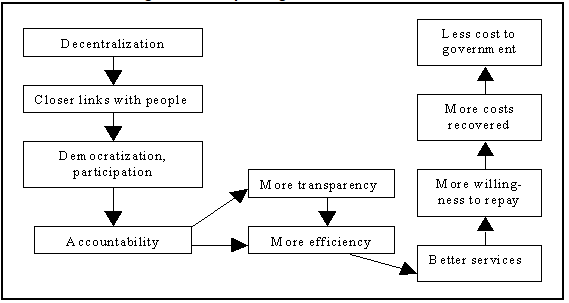
\includegraphics[width=0.8\textwidth]{Decentral.png}
    \caption{ Advantages of Decentralization of Governance }
    \label{fig:Advantages of Decentralization of Governance}
\end{figure}

% [image source - http://www.fao.org/docrep/005/y2006e/y2006e05.gif]

Consequently, the designed application will be used by the volunteers for the easy dispersal of information to the local people. People will remain informed about the ongoing government schemes, daily livelihood services and other local news. Participation in the ongoing surveys will also be managed and tracked easily. Delegation of community monitoring in the hands of volunteers will help in achieving the decentralization of governance effectively. 

\section{Literature Review and Related Work}
India is witnessing a phenomenal increase in mobile phone usage particularly in rural India over the last few years. Mobile handsets have become affordable and feature-rich making them amenable to value added applications. There is a consensus among mobile service providers, mobile content developers, banks and other financial institutions, policy makers (i.e., Reserve Bank of India, Ministry of Panchayat and Rural development), and various regulators (i.e., Telecom Regulatory authority of India, Indian Banks association, Insurance regulator of India, Mobile service provider association) that mobile applications is a viable way to reach information and service to rural people. The following papers were reviewed while developing the concept.

\begin{itemize}

\item Emergent Practices Around CGNet Swara, A Voice Forum for Citizen Journalism
in Rural India, ICTD’12 \cite{cgnet} : This paper talks about the initiative of CGNet Swara,
which is a project similar to JMR active in Chhatisgarh. The authors explain the
deployment of the system, and their experiences. It also delves into qualitative
and quantitative analysis of the data coming in, of the callers, topic about which
stories were reported among other things.

\item Designing Mobile Interfaces for Novice and Low-Literacy Users,ACM Transactions
on Computer-Human Interaction. 2011 \cite{design}: This study explores different interfaces
for low-literacy and novice mobile users. The authors conducted two studies com-
paring text-based interfaces to other different alternatives such as, one: automatic
solutions including graphics, spoken dialog and text-free user interfaces and sec-
ond: a live human operator. Based on these studies and interviews conducted
with the subjects, the authors cite results regarding the comfort of novice users
with the different mobile interface components. They also lay down certain design
recommendations while designing mobile user interfaces for such users.

\item Citizen Connect SMS Mobile Application \cite{Decen5:online} : This mobile application empowers citizens with access to information and grievance redressal of local government services.SMC was launched to provide latest information and facts to people and take the government services to the doorsteps of the citizens. They launched a mobile app ‘Citizens Connect’ that enables information sharing and service providing through latest technology.  The mobile app, which can be downloaded free of cost on Android phones, provides information regarding elected and administrative wings, registration procedures, recruitment advertisements and even rainfall. Users can also check birth and death certificate details, property tax details, pay water meter bills and share feedback. Having launched in 2013, the app has already received over 18 million service requests and 7400 complaints.


\item Mygaon, Web Platform \cite{MyGao25:online} : The initiative is centered around India's 6.4 lakh villages, and more importantly, their efforts towards ensuring that each of native village is prosperous, healthy, and safe place to live. Mygaon's vision is to create a comprehensive, dynamic and interactive web platform of information on villages in India in order to facilitate impactful and accelerated social change. On My Gaon, one is able to browse through real-time information on villages in India in a rich and visual manner. One can also view information regarding verified organizations which are involved in successful and highly impactful projects in these locations. They introduce 'Village Champions' - individuals on the ground who are willing to help community people make a lasting impact in the villages and thus provide them with all the information, tools and networks one need to contribute to one's native village.

\item Rural ICT \cite{home21:online} : Rural Information and Communication Technology (ICT) is a software platform that leverages cheap mobile phones and opportunistic Internet access for commercial purposes as well as group-based knowledge exchange. Users interact with the platform by dialing a phone number and navigating simple automated prompts using touchtone keys. It is a knowledge sharing system built for telephony, which empowers its users to engage in conversation, trade or exchange of ideas in any language and with any community, thus surmounting literacy and language challenges. The voice portal is a 24-hr system where customers can record their order any time, it will thus help in saving time, effort and money. Orders placed would be easily manageable, can be tracked and avoid any loss or missing orders. There is no limitation on no. of user availing this facility in a group and thus also can be used for public surveying. This automating of job is to set an online system to process transactions and announcements.

There are three users of the system named as admins, publishers and the members. The customers register to the system as members. The publisher along with the permission of the admin will handle the system and broadcast messages to respective customers.The members of the system, the customers can place their request on the system. It may be in the form of an order, a feedback or a response. All their response and request will be stored in the system and the publisher or the admin will make sure that the order is being processed successfully. Thus with the help this system, one can record a message (special offers or notifications) to be broadcasted.

\item Comparing Semiliterate and Illiterate Users Ability to Transition from Audio+Text
to Text-Only Interaction, CHI’09 \cite{findlater2009comparing} : In this paper, the authors establish fact that
illiterate and semi-literate users can’t be both clubbed together into one category
when it comes to designing suitable user interfaces for them. This is so because for
users with some basic literacy, who though might not be able to read and write flu-
ently, text provides an unambiguous mode of interaction. The authors conducted
studies where they found that when semi-literate users were presented with an
interface with both text and audio support, they soon reduced their dependence
on audio while no such improvement was found in case of the fully illiterate users.
The paper provides interesting insights into the differences in the responses of fully
illiterate and semi-literate users to different UI components.
\end{itemize}




\chapter{Landscaping Study}

%Replace \lipsum with text.
% You may have as many sections as you please. This is just for reference.
Before building any technology, we must explore the existing technologies of the same domain, their challenges and drawbacks, accessibility of these technologies to the target people and scalability issues. Many questions came in our mind before we started working on the solutions for information reachability to the community poeple.

\section {On Ground Surveys}
We conducted on ground surveys in the information deprived and backward areas of Delhi to find the answers of various questions. What type of problems are generally faced by these people? How people use media and mobile phones for solving their community level grievances? How people gain access to daily information, get their complaints solved, receive benefits of Governemnt schemes? How is government involved in solving these matters? How the grievances are amplified which forces government to solve the problems? We tried to find the answers of these questions by conducting following on ground surveys.

\begin{enumerate}
\item \textbf {Survey of ‘Munirka Village’}

Munirka is an urban area in South West Delhi, located near Jawaharlal Nehru
University (JNU) and Indian Institute of Technology Delhi (IIT Delhi)
Campuses \cite{Munir91:online}. Munirka is a village where development has started in early 1990’s.
The area is mostly dominated by the jaat community. We entered in a dealer’s shop
and asked about the village life, sarpanch and marginalized group in munirka.

Moreover, we found that the sarpanch of munirka himself lives in “Vasant Kunj”
and rarely visits his constituency. That was very disappointing part as he was not
at all involved in solving the problems faced by his people. He also gave us contact
number of vice-sarpanch “Bharat Singh” who lives in a nearby street in munirka.
He said “Munirka is no longer a village and the area was well developed where
everyone owns a smart phone and living a standard life. All shop owners were well
equipped with basic amenities. We also talked to some local shop owners on the
main street. The place was still following the village third-tier Panchayati Raj
System. Some points are summarized below.

\begin{enumerate}
\item It is now termed as an urban area but the place still follows the hierarchy of
sarpanch, vice-sarpanch and community people.
\item Shop owners were using TV as their source of information. Some youngsters
were listening to the radios for infotainment.
\item Government involvement was very less in their grievances.
\item People own the shop and had the information of their residence and their
area.
\item Many people own the mobile phones and there is good internet connectivity. We analyzed that by giving training to some responsible community people we can deploy this model in their community.

\end{enumerate}

\item \textbf {Survey of Vasant Vihar}

Our next visit was towards Vasant Vihar. Vasant Vihar is an exclusive
neighborhood located in the South West Delhi district of National Capital Territory
of Delhi. We had a visit to "Coolie Camp" situated in the same place. It is a slum area
where people were living in adverse conditions. There was no proper sanitation
facilities and no hygienic conditions. More than 3000 slums (jhuggi-jhopdiyas), cemented houses were agglomerated in such a small area. The irony is “Vasant Vihar is one
of the expensive residential areas in the world”  and it
still has such slum areas.\\

Well, we asked various questions to the residents of that place regarding the
availability of basic amenities. Whether they are able to avail the benefits of various
schemes, are able to solve their problems at community level, or by the involvement
of the MLA of their area “Parmila Tokas”. They said for the issues of water and
electricity availability, they approach to the MLA’s office to put their problems.
Sometimes, Officials or people from some department or ministry come to take
surveys for various statistics related to literacy rate, population count, number of
schools, toiletries etc but problems of local people are not addressed. They take
numbers and put it in records. One of the person standing near the retail shop said
that they make no efforts after the surveys, just take the figures that too improper
and report to higher authorities. People were reluctant in answering the questions and were uninterested in sharing
the stories and experiences they face and encounter.

\begin{enumerate}
\item  Women were dependent on male members of their family, were unaware of the community information and were carrying no mobile phones.
\item Youngsters were carrying the smart phones for receiving and making calls
and were using it generally for two applications i.e. Facebook and Whatsapp.
\item Local shop owners of the slum areas were carrying basic phones.
\item People aged between 40 to 60 were using phones mainly for gas booking
purposes and for receiving and making incoming and outgoing calls
respectively.
\item Youngsters wanted job related information.
\item No one was much concerned about health problems and health grievances.
\item People rely on words of their peers. Local people generally got informed from
mouth to mouth communication by their peers.
\item Shop owners are aware of their locality, its problems but have no smart
media and were seemed pre-occupied with their own local problems.

\item Skilled people having mobile phones can be given on ground training to learn the usability of application to address the above mentioned community problems.

\end{enumerate}


\item \textbf {Survey of Seemapuri}
Seemapuri is mainly a rural zone in Delhi. New Seemapuri is situated at one end of north east Delhi. It has Uttar Pradesh as border on one side and lies adjoining to Dilshad Garden in East Delhi. It is basically a heterogeneous community with multi-cultural, multi-lingual and multi-characteristic features. Most of them earn their bread and butter by picking and sorting of rags. Some are daily wage earners, street vendors, domestic helps, and many other menial jobs which are the main stay of their sustenance. Few of them are also shopkeepers, rickshaw pullers and semi skilled labourers working in the construction sector. The fact remains that many of the families are unable to feed their children with the meagre earnings they make.
\begin{enumerate}
\item There are two slums near dilshad garden metro station, Rajeev camp and Sonia camp which were earlier displaced from some other area of Delhi to Dilshad garden due to ongoing construction.
\item Rag pickers earn their wages by picking and selling waste material which is too less for their livelihood.
\item No government surveillance and cleanliness of the locality is maintained.
\item People are poorly literate and have no source of information to participate in social development and governance related activities.

\item NGO 'Action India' is located near the slum area of Seemapuri. We can select these people as HAPs to solve the local problems through mobile application.
\end{enumerate}

\end{enumerate}


\section{Visit to NGOs}
A non-governmental organization (NGO) is a not-for-profit organization that is independent from states and international governmental organisations. They are usually funded by donations but some avoid formal funding altogether and are run primarily by volunteers. NGOs are highly diverse groups of organizations engaged in a wide range of activities, and take different forms in different parts of the world. We talked to NGO personnel of 'Action India' working in Seemapuri Area for the cause of community peopel and for solving their  community and livelihood problems. 
\begin{enumerate}
\item \textbf {Visit to Action india}
Action India founded in 1976, has taken many big and small path breaking initiatives by grassroots women, which clearly indicates the strong potential in women to become change agents in the process of social transformation. Action India sustains a balance between community based work and the universal struggle for women’s rights. While protesting against wrongs, Action India simultaneously creates alternative modes of self-help, self-esteem and self-assertion.

We had a talk with Mr. Praveen from Action India, project co-ordinator Mr. Deven
and Mr. Pramod regarding Action India's approach in solving problems of women
and various programs like 'Women helping women', 'Save the girl child campaign', 'Adolescents-Education for equality', 'Access to water and sanitation', 'Rural Program - looking through a gender less'. Various sanghs like 'Sable mahasangh maitreyi mela', 'Hinsa mukt mahilaye', 'Beti utsav' were started and are being run.

The NGO works for women empowerment program. We have discussed the ways they follow to solve the problems of women.

 \item \textbf{Cause of Action India}
\begin{enumerate} 
 \item   \textbf{Eliminate Discrimination} : Action India initiated the Mahila Panchayat (women’s courts) as a forum for
dispute resolution and realized need and effectiveness of women’s support groups. With the help of legal resource persons the paralegal workers trained the mahila panchayat members on legal rights of women with a strong focus on gender equality. Paralegal workers from the community, mobilized members for the mahila panchayats and today we have 9 mahila panchayats in Delhi. Mahila Panchayat has 14 paralegals and 225 mahila panchayat members. Mahila Panchayats themselves involve in solving the issues of women and support all the cases without any bias till the end.

 \item \textbf{Facilitate access to education} : For education related issues, they approach to School Management Committees, Dept. of School Education and Literacy, Ministry of Human Resource Development, Government of India which sometimes involve in solving the teacher absenteeism problem, School Mgmt Team, Mid day meal Distribution etc.
 
 \item \textbf{Facilitate access to health care} : They approach to health and sanitation committee where they force them to solve
the issues, go to deliver reports in person, for complaints they seek for constant reports and keep receiving to show in case they don’t entertain. NRHM benefits are also seeked by people.

 \item   \textbf {Enhance access to livelihood and economic rights} : Near the New Seemapuri Road which is approx. at 1 km distant from the Dilshad garden metro station, the complete road is occupied by the rag pickers (kabadi vala)
with their sacks. Due to this, this road smells very much and the residents have
problem with it. But as the Action India volunteer Mr. Praveen told us, this work is
the only livelihood for these rag pickers. Also, the MCD vehicle cleans all the
leftouts by the rag picker daily in the evening. We talked to the rag pickers also
asking the problems faced by them and how do they get it solved. We found from the
conversation that their voice is not heard by anybody nor it is communicated to the
govt. authorities.
When they were told about the android application features, they found the
grievance redressal the most useful. As their primary need is to secure their
livelihood and not the secondary needs which they cannot even think to access.
 \item  \textbf{ Enable participation in governance and development} : They encourage people to participate in the local governance related and development issues of society.
\end{enumerate}

\pagebreak
\item \textbf{Conclusion} After having a healthy discussion with amy people in NGO, we came to know that they are willing to address the problems of their community people. They are ready to willingly help the society by participating in this system.
\end{enumerate}




\section {Observations and Suggestions}

\begin{enumerate}
\item Political Agenda for all the commissions matters more than the actual solution for the problem.
\item School Association Committee (SMCs), health and sanitation committee (HSC) were not able to solve and address the villagers problem effectively.
\item Recognizing and delivering on-ground training to Human Access Points is very essential for the model.

\item On-ground training is mandatory before launching any scheme, giving any
benefits, introducing ICTD media among people, deploying any technology.
\item Manual intervention and involvements are the key elements in introducing
big changes and turning heads of the people.
\item The local knowledge of village is very important prior to introducing any new
model in that place.
Necessity of responsible people in various regulatory authorities, commission
departments, panchayats, Government officers, NGO’s workers, ASHA
workers, school teachers.
\item People should themselves come forward to seek solutions and seek
information and registering complaints.
\item There are many mobile phones users and they can be given training for
making the human access points and local villagers known with the problem
and the technologies.
\end{enumerate}

\section {Conclusions}
It is analysed from all the surveys that people who live in the underdeveloped areas
like rural areas and the slums do not have a platform where they can get all theinformation about the basic needs which they require in their lifestyle. Information
about administration, education, health schemes, employment, agriculture, gas
cylinder bookings, land acquisitions can be correctly communicated to them which
will help them on fulfilling their needs and eventually develop and making their
lifestyle better. But there are certain problems in the implementation of the
method.

\begin {enumerate}
\item  People do not have even small knowledge of operating the mobile phones
whether basic mobile phones or smart phones. Condition is even worse with
women. Though youth and earning member of the house have phones but
still they do not know more than dialing and receiving the call thus intense
training is required for the proper implementation of the approach.
\item  People are reluctant in sharing the information to the people outside their
community. Or they tell data which is partially or completey false. Thus to
collect data through telephonic surveys, Trust needs to be built that it is for
their welfare only.
\item If started by implementing the approach for all the areas mentioned above, it is likely that it will be implemented properly for all the fields and a large dataset of information is required and need to be maintained. Thus the approach should be started by implementing for 1 or 2 areas initially.
\end {enumerate}



\chapter{System Architecture}

\section{Platform and Technologies Used}
\subsection{Application Server}
\begin{itemize}
\item \textbf{Framework : Ruby On Rails}\\
Ruby on Rails is a web application framework written in Ruby under the MIT License. Rails is a model–view–controller (MVC) framework, providing default structures for a database, a web service, and web pages. The complete framework can be easily setup on system using the following links \cite{Setup43:online} \cite{RVM:R7:online}.

\textbf{Ruby version} : ruby 2.3.0p0 (2015-12-25 revision 53290) [x86\_64-linux] \\
\textbf{Rails version} : Rails 4.2.6

\item \textbf{Network Library} \\
\textbf{RestClient} : A simple HTTP and REST client for Ruby, inspired by the Sinatra microframework style of specifying actions: get, put, post, delete \cite{GitHu91:online}.\\
\textbf{Net::HTTP} : A rich library which can be used to build HTTP user-agents. It is designed to work closely with URI::HTTP\#host, URI::HTTP\#port and URI::HTTP\#request\_uri  \cite{Class28:online}.
\item \textbf{Database} : MySQL Server \\ 
\textbf{MySQL version} : mysql  Ver 14.14 Distrib 5.5.49, for debian-linux-gnu (x86\_64)
\item \textbf{Web Server} :  Puma\\
Puma is a library that provides a very fast and concurrent HTTP 1.1 server for Ruby web applications. It handles multi threading by running multiple worker threads. The number of the threads running at an instant can be altered as per the load on the system \cite{AMode24:online}.\\
Puma version : puma version 3.4.0

\item \textbf{Push Notifications} : Google Cloud Messaging (GCM) Server
\end{itemize}


\subsection{Android Application}

\begin{itemize}
\item \textbf{Framework : Android Studio} \\
Android Studio provides the fastest tools for building apps on every type of Android device. Android Studio is freely available under the Apache License 2.0.

\textbf{Android Studio version} : Version of Android Studio 1.5.0 is used to build the application \cite{Intro42:online}.

\item \textbf{Network Library} \\
Volley library makes executing asynchronous network calls, loading multiple images in the background, and response caching simpler. Android uses volley libraries for asynchronous task communication to the app server \cite{Andro34:online}

\item \textbf{Database} : SQLite \\
Android uses SQLite Database for storing information on phone.

\item \textbf{Android Software Development Kit (SDK)}\\
Minimum SDK build tool and Platform tool with APIs level 21 or above is required to support the working of various libraries on android phones.

\item \textbf{Receive Notifications} : Google Cloud Messaging (GCM) Client
\end{itemize}

\pagebreak
\section{System Flow}

Following Diagram depicts the entire System Flow.\\ \\ \\
\begin{figure}[H]
    \centering
	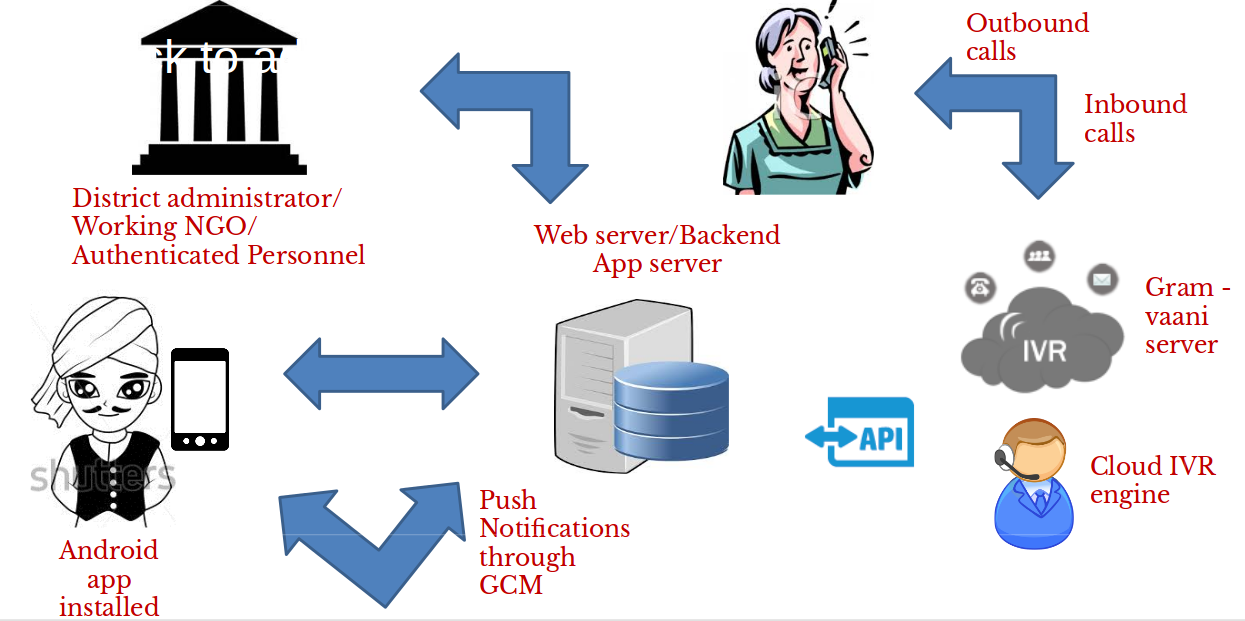
\includegraphics[width=0.8\textwidth]{Sysflow.png}
    \caption{System Flow}
    \label{fig:System Flow}
\end{figure}

\section{Use Case Diagram}
\begin{figure}[H]
    \centering
	\includegraphics[width=0.8\textwidth]{UseCaseDiagram.png}
    \caption{Use Case Diagram of Application User}
    \label{fig:Use Case Diagram of Application User}
\end{figure}

\pagebreak
\section{Entity Relationship Diagram}

Following Diagram depicts the entire database schema design.
\begin{figure}[H]
    \centering
	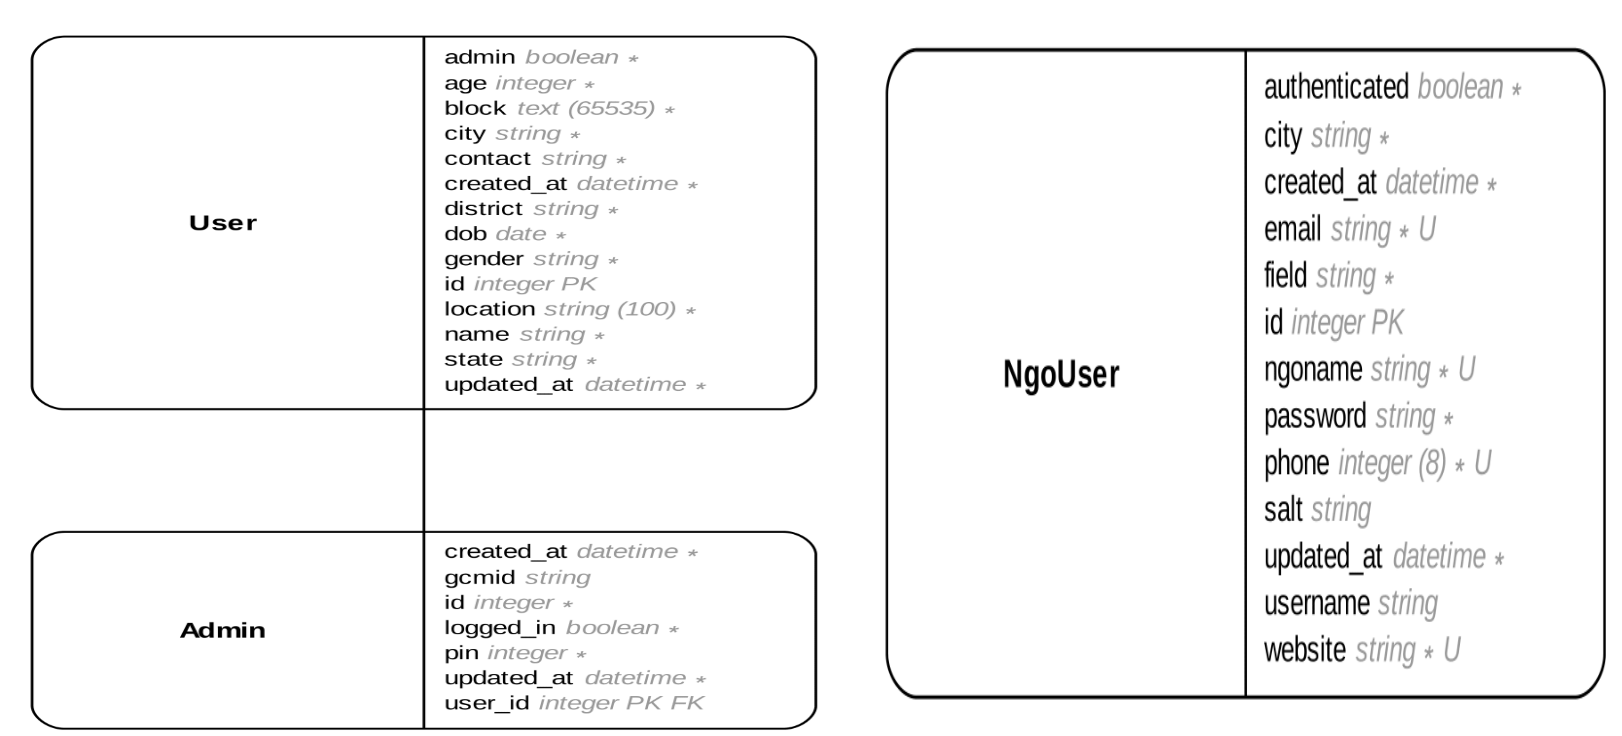
\includegraphics[width=1\textwidth,height=7cm]{erd1.png}
    %\caption{Entity Relationship diagram}
    \label{fig:erd1}
\end{figure}
\begin{figure}[H]
    \centering
	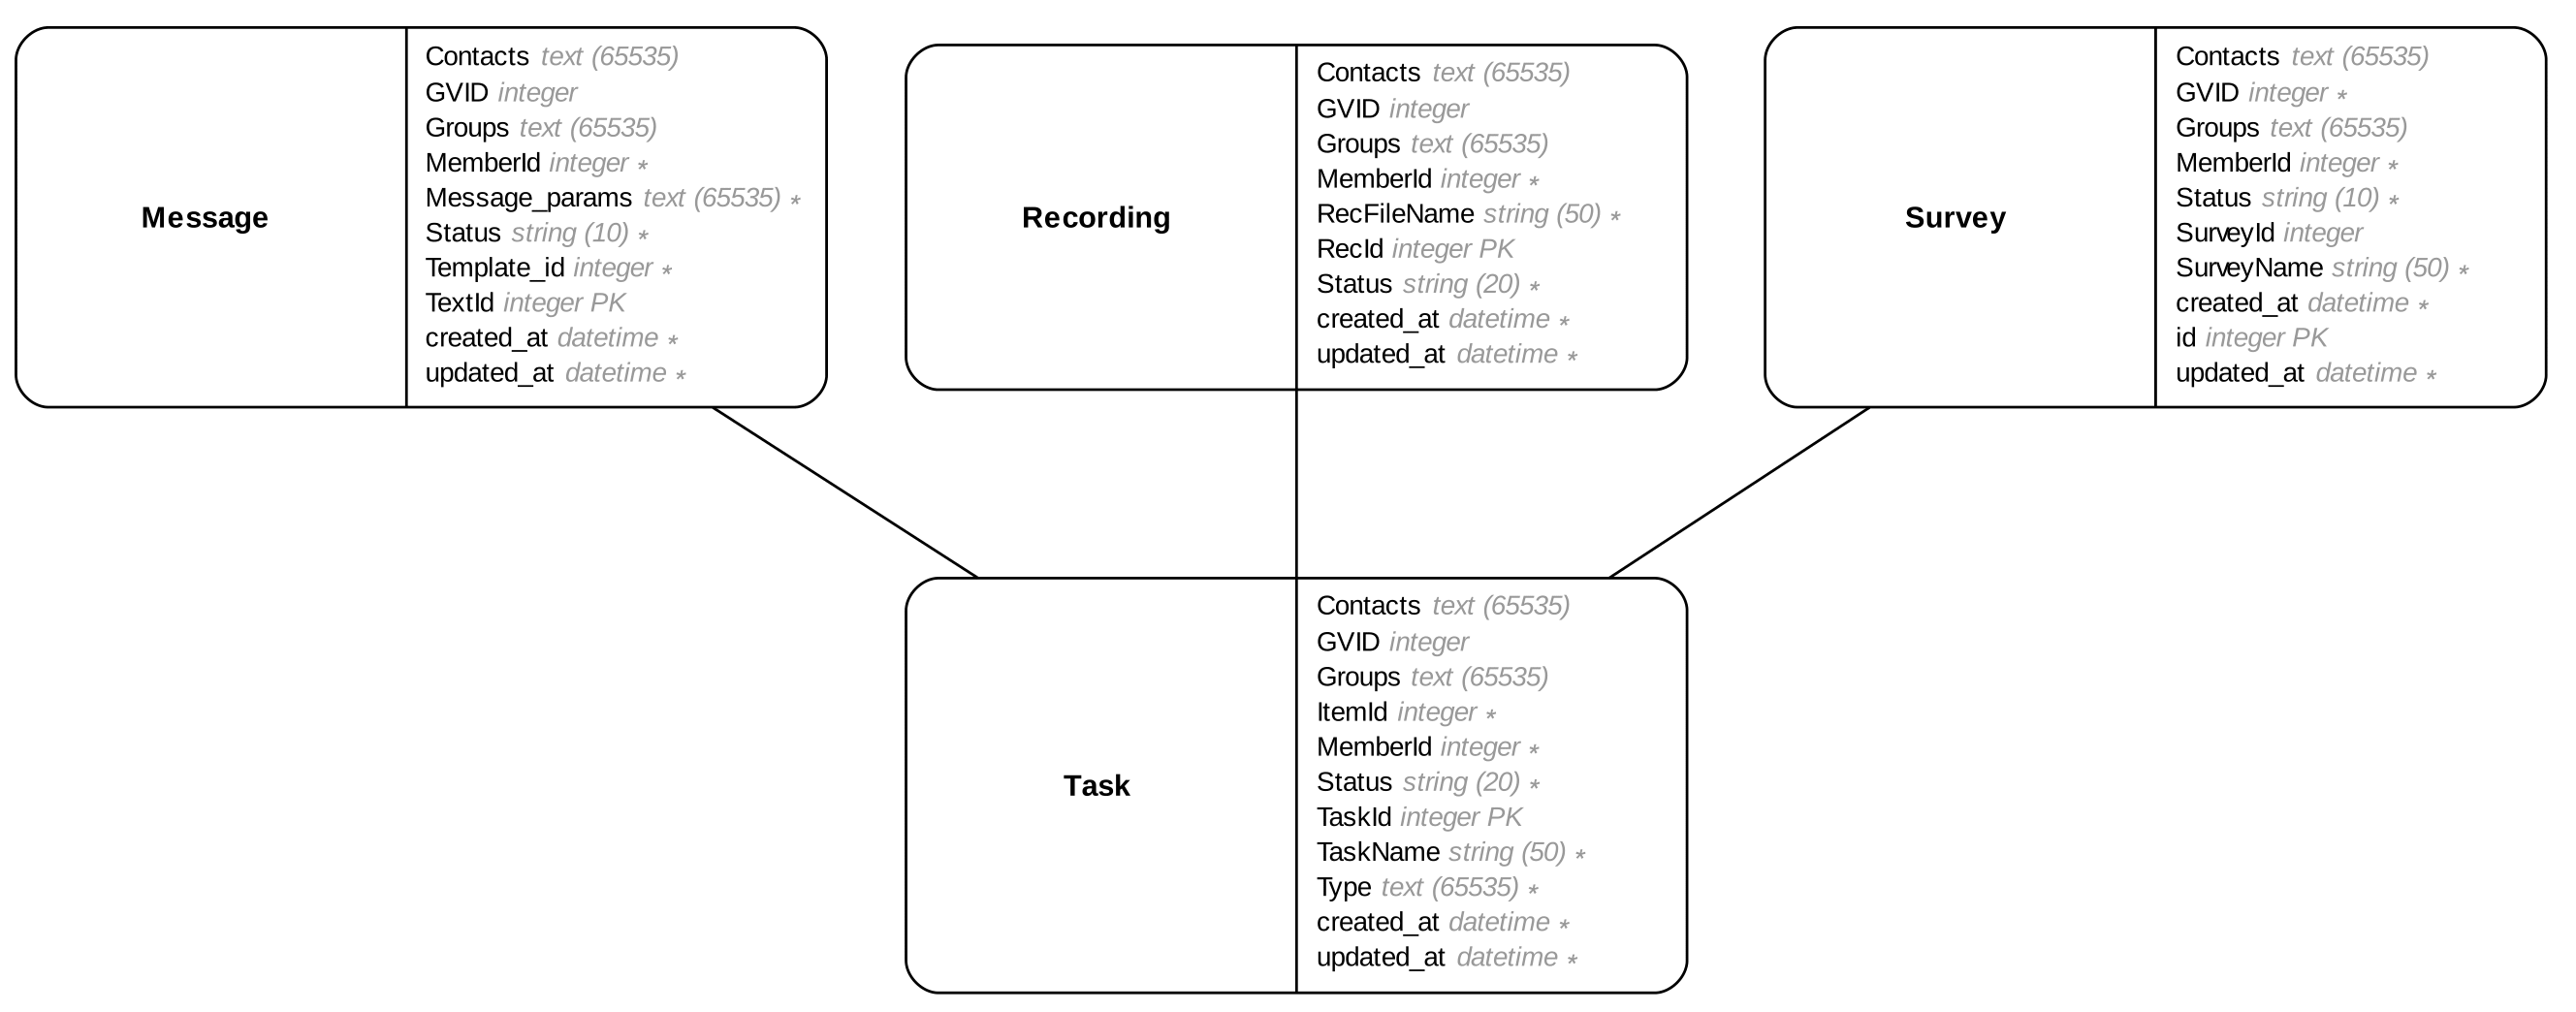
\includegraphics[width=1\textwidth,height=9cm]{erd2.png}
    \caption{Entity Relationship diagram}
    \label{fig:erd2}
\end{figure}
\section{Information flow}
Mobile Application is designed for the volunteers of the village. Along with, a portal is designed for the  NGOs/ Block or district officials for sending alerts to the volunteers of the community. Some volunteers from the community ( For instance, panchayat members, School teachers) will be chosen by the functioning NGO or block/ district administrator under which the community/ village falls. NGOs/ Block or district officials will give authorization to the selected volunteers from that community by registering them through the portal. After authorization, volunteers will be given an Android phone installed with the local governance application "Gologo". Credentials of volunteers will be authenticated on first time login in the application. After successful one time login, volunteers aid their local community people by exploring the app functionalities. Portal will be used to send survey alerts to the volunteers. Volunteers will receive alerts  on their mobile phones to further disperse it to the target people. Through this way, information will flow by the people and  among the people via various functionalities.

%Following Diagram depicts the flow of information through \hyperref[itm:launchsur]{Launch Survey Use Case} whcih is explained later.

%\begin{figure}[H]
 %   \centering
	%\includegraphics[width=0.9\textwidth]%{launchsurvey1.png}
  %  \caption{Launch Survey Use Case}
 %   \label{fig:Launch Survey Use Case}
%\end{figure}
%

%\include{chapter4}

\chapter {Local Governance Application}

%Replace \lipsum with text.
% You may have as many sections as you please. This is just for reference.
\section{What is Gologo?}

Gologo is an android operating system based local governance application which will provide the functionalities to volunteers for sending infotainment news and announcements to the local residentials of the community. Users (Volunteers) of the application will be able to broadcast news among localites in an easy and quick way.  The system provides platform to send quick audio and message updates to the relevant users. Volunteers will receive alerts regarding ongoing surveys from the authorized block/ district officials (through web portal)  on their application to launch surveys in their community. They can also track responses of the people for the surveys which are launched. Consequentially, System helps in delegating governance responsibilities to the community people in an effective and relevant manner.

\section{Application Flow}
 Entire flow of the application is explained through the application flow diagram. User interaction with the application is designed in a very simple way as application icons implicitly depict the functionalities. The sequence of activities is described by the below diagram.

\begin{figure}[H]
    \centering
	\includegraphics[width=1\textwidth]{eventflow1.png}
    \caption{ Application Flow Diagram 1}
    \label{fig:Application Flow Diagram 1}
\end{figure} 

\begin{figure}[H]
    \centering
	\includegraphics[width=1\textwidth]{eventflow2.png}
    \caption{ Application Flow Diagram 2}
    \label{fig:Application Flow Diagram 2}
\end{figure} 

\begin{figure}[H]
    \centering
	\includegraphics[width=1\textwidth]{eventflow3.png}
    \caption{ Application Flow Diagram 3}
    \label{fig:Application Flow Diagram 3}
\end{figure} 

\section{Functionalities}
The android application which is provided to the human access points/ volunteers of the society has the following features.
\begin{itemize}
\item \textbf{One Time Login} : After registration through the \hyperref[chap:ngoportal]{web portal}, volunteer receives a unique pin number of 6 digits on his registered mobile number. After installing the application, user has to do one time login. On first time login in gologo, the volunteer is authenticated for the application with his registered contact number and received PIN. On right credentials, volunteer can directly use all the functionalities as verification will be done only once. 
\ref{fig:pin_authenticate}


\begin{figure}[H]
    \centering
	\includegraphics[width=1\textwidth]{SDLoginData.png}
    \caption{ Sequence Diagram of User Login }
    \label{fig:Sequence Diagram of User Login}
\end{figure}

Also, on first time login. GCM registration on GCM server will be done and user receives a unique registration ID. This registration ID will be used to send alerts to the user. Also, all requests to the app server involves the authentication through the obtained registration ID. The uniqueness of the registration ID will help in authenticating the user via taking registration ID as key \hyperref[GCMlink]{obtained by GCM}. 

\item \textbf{Pin Recovery} : User can ask for the PIN in case the user forgets the received pin. He will click on forget pin option provided on the login screen. A text message containing the pin will be received which can be used for one time login into the application for the authorized volunteers \ref{fig:pin_recovery}.

\begin{figure}[H]
    \centering
	\includegraphics[width=1\textwidth]{SDPinrecovery.png}
    \caption{ Sequence Diagram of PIN Recovery}
    \label{fig:Sequence Diagram of PIN Recovery}
\end{figure}


\item \textbf{Broadcast Announcements} : After authentication from the server into the android app, the user can select the option of Broadcast Audio on the home screen. Under this option, the app user gets a recording screen through which he/she can record an audio message of any instant broadcast. Then, contacts picker screen \ref{fig:contactoptions} appears through which he can select the either of the following options :

\begin{itemize}
	\item Concerned multiple Gramvaani groups \ref{fig:contactgroups}.
	\item Local contacts saved in phone \ref{fig:phonecontacts}.
	\item Mobile Vaani callers between a  particular duration.
\end{itemize}

\begin{figure}[H]
    \centering
	\includegraphics[width=1\textwidth]{SDLaunchAudio.png}
    \caption{ Sequence Diagram of Broadcasting Announcements }
    \label{fig:Sequence Diagram of Broadcasting Announcements}
\end{figure}


After selecting a particular option, he chooses the target people and clicks on button. After clicking on send button, a request to the app server is made to send the audio. The message will be then sent to the contacts through Gramvaani voice calls. Application user will receive an alert  message through the GCM notification when message gets played to the target audience.
Recorded audio message will be saved in the mobile vaani instance as content so that people can later listen to it when they give calls to the IVR.

\item \textbf{Survey Dial Outs} \label{launchsur} : Volunteer acts as a bridge between the NGOs/District officials etc to make the surveys available to the end people. Results will be notified to both the admins through application and NGO personnel through the website. User gets a list of all active surveys mapped to different application instances from which he can choose one particular survey to launch in the community \ref{fig:viewlaunchsurvey}.

\begin{figure}[H]
    \centering
	\includegraphics[width=1\textwidth]{SDSurveyList.png}
    \caption{ Sequence Diagram of Getting Active Surveys}
    \label{fig:Sequence Diagram of Getting Active Surveys}
\end{figure}


Volunteer  chooses this option to launch the survey in his community. A request will be sent to the application server having the authenticated GCM registration ID to get a list of ongoing recent surveys from the Gramvaani server. Each listed survey will have the following options:
	\begin{enumerate}
	\item{ View Survey} : Volunteer can view the questions of a particular survey. When volunteer selects a survey, the unique survey id along with the authenticated credentials will be sent to the application server. Application user gets a list of text questions along with the type of question and audio prompts of the survey.  \ref{fig:viewsurvey}.
	
\begin{figure}[H]
    \centering
	\includegraphics[width=1\textwidth]{SDViewSurvey.png}
    \caption{ Sequence Diagram of Viewing Active Surveys}
    \label{fig:Sequence Diagram of Viewing Active Surveys}
\end{figure}

	\item{Launch Survey} : Volunteer can launch a particular survey in his community via two ways.
	
\begin{enumerate}
	\item\textbf{On receiving GCM notification} : NGO/ District official are provided with the functionality on the web portal to send GCM notifications to the registered users \ref{fig:Launch Survey Step 1 on the Web Portal} \ref{fig:Launch Survey Step 2 on the Web Portal} . List of surveys will be displayed to the NGO personnel. He will select a particular survey and the location where survey is to launched. Depending upon the selected location, portal displays a list of registered volunteers. He will select the volunteer and click on send which will send a GCM notification alert to the respective volunteer on his application. Application user clicks on notification to launch that survey by sending a list of relevant contacts to the application server.


	\item\textbf{On pressing launch button on application} : By clicking on launch button, volunteer is provided with the contact options where he will choose the list of contacts from the given options. A request with survey id and list of contacts  will be sent to the application server for the dial outs.

\begin{figure}[H]
    \centering
	\includegraphics[width=1\textwidth]{SDLaunchSurvey.png}
    \caption{ Sequence Diagram of Launching Active Surveys}
    \label{fig:Sequence Diagram of Launching Active Surveys}
\end{figure}
	\end{enumerate}


\item {View Survey responses} :  This functionality is provided to view the status of launched survey. Volunteer can track the number of people who responded the survey calls. Application also lists the count of responses corresponding to each question. In survey dial outs, it is possible that receiver won’t respond to all questions and cut the call in between.  In that scenario, volunteer also gets the statistics of responses per question. It will help him in acknowledging the survey status. He can also send the message alerts to the community regarding survey reminders. 
\end{enumerate}

\item\textbf {Send text Alerts} - Similar to the audio message, the user can
send a text message to the selected contacts \ref{fig:contactoptions}. The user selects the Send
message button from the home screen, selects the contacts/groups from
one or more of the three options described above and sends the message
which then makes a request to the app server to send the message to
the selected contacts through Gramvaani server. Templates are registered with the Gramvaani where volunteer will feed only the values related to a particular template. It helps in informing end users instantly regarding the news of surveys, government schemes or future camps nearby their locality area. Following templates are used to send text message alerts to the target people \ref{fig:message}.

\begin{figure}[H]
    \centering
	\includegraphics[width=1\textwidth]{SDLaunchmessage.png}
    \caption{ Sequence Diagram of Launching Message}
    \label{fig:Sequence Diagram of Launching Message}
\end{figure}

\begin{enumerate}
\item \textbf {Template for Announcement of surveys} - Text alert of survey to be launched in the community will be sent with the specified date to inform people regarding the survey launch. Application user selects the date of launching using date picker. Selected value will be fed in the template \ref{fig:message1}.

Input Params: date 

Message Template (English) : Dear all, a Survey ​will be launched in your village on date $\langle date \rangle$  by Mobilevaani. Please submit your responses sincerely. ​Team Mobile Vaani.
 
Message Template (Hindi) : Priye nivaasiyon​, mobile vaani dwara ​ek sarvekshan dinaank $\langle date\rangle$  ko ​aapke​ gaanv mein shuru kiya jaega. Kripaya apni pratikriya ​jaroor​  prastut karen. Team Mobile Vaani.

\item \textbf {Template for Announcement of Camps (with timings)} - Text alert of upcoming camp to be organised in the community will be sent with the specified parameters to inform people. Application user selects the parameters from the drop down and insert the values in edit text date of launching using date picker. Selected value will be fed in the template \ref{fig:message2}.

Input Params: campname,  startdate, enddate,  starttime, endtime, venue
 
Message Template (English) : $\langle campname \rangle$ Camps will be organized at $\langle venue \rangle$  from ​date $\langle startdate \rangle$  ​to $\langle enddate \rangle$  with timings from $\langle start time \rangle$  to $\langle end time \rangle$ . Kindly participate in the camp to take​ its maximum benefits. Team Mobile vaani.

Message Template (Hindi) : Priye nivaasiyon​, $\langle campname \rangle$  camp $\langle venue \rangle$  sthaan par dinaank $\langle startdate \rangle$  se $\langle enddate \rangle$  ko samay $\langle start time \rangle$  se $\langle endtime \rangle$  tak aayojit kiya jaega. Kripaya camp mein bhaag lekar iska adhiktam laabh uthae. Team Mobile vaani. 


\item \textbf {Template for Announcement of Camps(without timings)} - Text alert of upcoming camp to be organised in the community will be sent with the specified parameters to inform people. Application user selects the parameters from the drop down options and insert the values in edit text. Selected values will be fed in the template \ref{fig:message2}.

Input Params: campname, startdate, enddate, venue

Message Template (English) - $\langle campname \rangle$ Camps will be organized at $\langle venue \rangle$ from ​date $\langle startdate \rangle$ ​to $\langle enddate \rangle$. Kindly participate in the camp to take​ its maximum ​benefits. From Team Mobilevaani.
 
Message Template (Hindi) - Priye nivaasiyon​, $\langle campname \rangle$ camp $\langle venue \rangle$ sthaan par dinaank $\langle startdate \rangle$ se $\langle enddate \rangle$ ko aayojit kiya jaega. Kripaya camp mein bhaag lekar iska adhiktam laabh uthaen.Team mobile vaani.

\item \textbf {Template for Announcement of Govt. Schemes} - Government Schemes which are launched can be notified to the community people via this template alert \ref{fig:message3}.

Input Params: schemename, date, beneficiaryname 
    ​
​Message Template (English) - Dear all, Government has launched $\langle schemename \rangle$ Scheme on date $\langle date \rangle$ for $\langle beneficiaryname \rangle$​. For more information, contact the volunteers ​and take​ its maximum ​benefits. Team ​Mobilevaani. 
 
Message Template (Hindi) - Priye nivaasiyon​, sarkaar dwara $\langle schemename \rangle$ yojana dinaank $\langle date \rangle$ ko ​$\langle beneficiaryname \rangle$ ke lie ​shuru ki gai hai. Adhik jankari ke lie volunteers se sampark karen aur iska adhiktam laabh le.Team mobile vaani.
\end{enumerate}


\item \textbf {Add a group} - Volunteers are given this functionality for the management of contact groups. Multiple contact groups are made and managed as per the groups of the community. It helps in easy dissemination of information to the relevant audience. App user can speak group name where his voice will fill the text view. When user clicks on create button, new contact group with that name will be created in the corresponding application instance. \ref{fig:group1}.

\begin{figure}[H]
    \centering
	\includegraphics[width=1\textwidth]{SDAddGroup.png}
    \caption{ Sequence Diagram of Adding a Group}
    \label{fig:Sequence Diagram of Adding a Group}
\end{figure}

For example, if some polio booth camp is to be organised in the community, then only the relevant people who have children of age 3-5 should be informed instead of unnecessary sending dial outs to all people.

Similarly, Survey regarding death due to pregnancy will be sent to homes having women. Dial out will be made to only those contacts/ contact groups who falls in this category. Global surveys can be sent across all groups which are relevant to all people of the community.

 \item \textbf {Add a contact} - The app users can add a new contact. The user selects the option of add a contact on the  home screen of application. In this option, he can fill in all the details of a new contact of his community having name, contact number, gender, date of birth, contact groups and location URI. Volunteer need not to type the name of the contact. He can simply speak the name of the person by clicking on speaker image and it will be converted into text. Phone will be a ten digit mobile number. Gender is a drop down menu containing ‘F’ and ‘M’ as the options. Date of Birth can be chosen using date picker. One contact can be added in multiple  contact groups. Contact groups are fetched from the Gramvaani instance. Application user gets a check list having all existing contact groups where he can select one or more groups to add contact in it. Locations are also fetched from the Gramvaani database where each location contains block, district and state \ref{fig:contact1}.
 
Volunteer fills all the details from the options into the text boxes and spinners. When he clicks on create, a dialog box asking for confirmation pops up. He can either click on edit to change any detail or on confirm to add the new contact \ref{fig:contact2}.

When volunteer clicks on confirm, a request having json data will be sent to the  Gramvaani server from the application server to update its contacts through APIs. In json data, location URI corresponding to each location will be sent. Also, block, district and state will be extracted from the displayed locations and sent separately. Similarly, ids of the contact groups corresponding to each contact group name will be sent. In a way, json data will be sent to the server in terms of key value pairs.

\begin{figure}[H]
    \centering
	\includegraphics[width=1\textwidth]{SDCreateContact.png}
    \caption{ Sequence Diagram of Creating New Contact}
    \label{fig:Sequence Diagram of Creating New Contact}
\end{figure}

 After confirmation, the app server sends added contact response. Thus, contacts will be synced from and to the Gramvaani server.

\section{Extra Features}

Some quick options on side action bar are provided on the application which are available across all activities. Application  user can navigate across these options. Following options are explained \ref{fig:menubar}.
\begin{enumerate}
\item \textbf {My Profile} - A volunteer can view all his details which are entered when he was registered through the portal. His details contains his user type, name, registered number, date of birth, gender, block, district and state.
\item \textbf{Home} - The user can directly go to the home screen from any screen.
\item \textbf{View contacts of a group} - User can view the contacts present in a particular group.
\item \textbf{Application Information} - This option enlists the usability of each option on home screen with a brief description. It helps the application user to know about the functioning of each option on menu.
\item \textbf{Gramvaani Website} - This option redirects the volunteer to the portal of the Gramvaani from the application.
\item \textbf{View Recordings} - Volunteer can view all the recordings he did directly from the application.
\item \textbf{Share Application} - Volunteer can share the link of .apk file of the application among the people using various options like Whatsapp, Gmail, Facebook etc. It sends the message along with the link to spread the word.
\end{enumerate}


\section {Usability}

Application can be used extensively to achieve various benefits. Volunteers will receive on ground training for the usability of the application. People will be taught regarding its usage and advantages. They will learn how these community people can be benefitted by it and how information can be disseminated among people by using it effectively. It will bring changes among the lives of poor people by equipping them with the tool of information. Their basic phones will be used to respond to the surveys, to view recent news, to receive text alerts, to listen audio announcements, to browse through the content by dialing to the mobile vaani. Following uses are listed below.

\begin {enumerate}
\item Volunteers can use the application to receive alerts sent by the NGO/ Block/ District officials.
\item Volunteers can use the application to send text alerts related to any recent news, entertainment shows, ongoing infotainment media  etc.
\item Information related to government schemes can be disseminated among the people.
\item Information related to community camps to organise in the society can be broadcasted through text alerts.
\item Instant audio messages to the relevant audience can be sent as dial outs by selecting concerned contact groups.
\item Contact groups can be managed which helps in easy handling of large target community. Groups like “Teachers”, “Farmers”, “Women”, “Children”, “Zamindars”, “Middle Man”, “ Wholesalers” etc can be created and maintained by adding new contacts among them properly.
\item One to one addressing is possible by sending dial outs to individual contact numbers which helps in gathering more responses from the people.
\item Survey responses will increase by separate dial outs which gives more realistic  survey results and accordingly, measures will be taken by the government.

\end {enumerate}

\section{Challenges and Suggestions}

The following are some of the challenges identified in the smooth run of the process. The ones listed below are primarily from the point of view of the application and target people where in spite of rigorous training and best interest and efforts of the community representatives, their contribution may be unworthy in helping the community people.

\begin {enumerate}

\item \textbf{ Poor internet connectivity}

The internet connectivity in the areas where the app is operated is often not good. Even though many a times there is network available on the phone, internet connectivity speeds can be very low. Due to no internet connectivity or slower speeds, there might be delay in the time when the text updates or dial outs are received at the community level. Also, large audio announcements in MBs will take more time to upload on the server and requires continuous net connectivity. On flaky networks, it will result in repeated failures while uploading. A continuous net connectivity will help in smooth uploading of the audio files. Rest, all functionalities require change of text data which will work in poor connectivity areas or when app user comes in affinity of the internet, data can be exchanged over the network.

\item \textbf{ Long Power Cuts}

A number of times, there are long power cuts due to which the Android phones cannot be easily charged again. Imagine a scenario where a community representative has to delegate some information to the community, but due to inability to charge the phone his phone got switched off before the updates can be sent. In such a case, updates won’t be received at the server till the phone is switched on again and gets proper internet connectivity. In order to deal with this, the community representatives were taught about simple steps to manage their battery. For example, keeping the phone brightness low, switching of apps which connect to the internet and regularly charging their phones whenever they have electricity. These are small precautions that can be taken to avoid a situation like above but it can still be a
cause of delay in sending information updates or dial outs to the community poeple.

\item \textbf {Novice Users}

Since the community representatives are novice smartphone users, a rigorous training is mandatory in which dealing with phone problems along with application usability is taught. Problems such as Message Memory Full or Phone Memory Full perplex them and they are not able to handle them. The way the phone functions is that you are not able to access anything on the phone until some memory is freed. In order to counter such situations, basic guidelines were given to the community representatives in written on how to handle such situations. But this can only be done for a few specific common problems. This is necessary as when these community representatives take their phones to a local shop to be checked, at times they delete certain applications. For instance, community representative may not be able to contribute for his community due to these issues in spite of best of intentions.

\item \textbf{Ignorance of Community People}

People among whom the news is disseminated may not be able to interpret it. They may not understand the audio or text message.  Illiteracy regarding the basic phones usability  like how to operate, how to open message box, how to pick phone etc can also hamper the information.  Also, Peoples’  behavior of not responding to the dial outs, cutting phone  in between, not willing to respond etc are major issues. Volunteers should keep themselves in touch with the people. Initial training session to teach  basic phone usability can be organised to train them.

\item \textbf{Volunteers unavailability}

Delay in information reachability, unawareness, absence of volunteers, social gap among volunteers are major issues. Multiple volunteers in a community  will ensure the availability of at least one volunteer. Volunteer sociable within the community must be appointed.


\item \textbf{Scalability and Multi-Lingual support}

App is designed in hindi and english. We have to  design app in regional languages to scale and diversify it which ensures wide variability.
\end {enumerate}

\end{itemize}








\chapter{NGO's Web Portal}
\label{chap:ngoportal}
Gramvaani Soochna Sanchar is a means for the NGO users and government officials to decentralize the governance by dividing the responsibilities and giving it in the hands of responsible people of society who are a part of it. These are literate, social and reputed people of the society and termed as \emph{Human Access Points} or admin volunteers. Human access points become a \emph{gateway}  with which the NGO personnel and government officials are able to disseminate information in the parts of society in which information circulation is not feasible due to various factors such as illiteracy, infrastucture, internet connectivity, multi-lingual issues and many other problems. NGO personnel and government officials can keep the information in a database of all the human access points at a location which is an easier task to do as compared to keeping the information of all the residents of the community. Through these human access points, NGO personnel can easily get the information of the whole community. Thus, it acts as an \emph{hierarchical architecture} to reach the farthest people of the community. NGO personnel can launch the tasks to the human access points which HAPs can communicate to the local people of the community. These tasks include \emph{Launching a survey}, \emph{Broadcasting an audio announcement} and  \emph{Circulating text message}. The web portal provides the above mentioned functionalities to the NGO personnel and government officials. In addition to this, NGO users and government officials can also view the information of the human access points at a location, active surveys, questions in a survey and responses submitted corresponding to the launched surveys. Web Portal Screenshots can be viewed in figure \ref{fig:Homepage part 1 on the Web Portal}, \ref{fig:Homepage part 2 on the Web Portal}, \ref{fig:Homepage part 3 on the Web Portal}.

\pagebreak
\section{Technical Specifications}

\begin{itemize}

\item \textbf{Framework : Ruby On Rails}\\
Ruby on Rails is a web application framework written in Ruby under the MIT License. Rails is a model–view–controller (MVC) framework, providing default structures for a database, a web service, and web pages. The complete framework can be easily setup on system using the following links \cite{Setup43:online} \cite{RVM:R7:online}.

\textbf{Ruby version} : ruby 2.3.0p0 (2015-12-25 revision 53290) [x86\_64-linux] \\
\textbf{Rails version} : Rails 4.2.6

\item \textbf{Network Library} \\
\textbf{RestClient} : A simple HTTP and REST client for Ruby, inspired by the Sinatra microframework style of specifying actions: get, put, post, delete \cite{GitHu91:online}.\\
\textbf{Net::HTTP} : A rich library which can be used to build HTTP user-agents. It is designed to work closely with URI::HTTP\#host, URI::HTTP\#port and URI::HTTP\#request\_uri  \cite{Class28:online}.

\item \textbf{Webpages} \\
The views(can also be termed as webpages) are designed using \\
\textbf{HTML} (HyperText MarkUp Language). \\
\textbf{CSS} which is abbreviation for Cascading Style Sheets  is a language used for describing the presentation of a document written in a markup language. \\ 
\textbf{JavaScript} to add client-side behavior to HTML pages. \\
\textbf{Bootstrap} is used for setting the structure of the website using its templates, themes and form helpers.

\item \textbf{Database} : MySQL Server \\ 
\textbf{MySQL version} : mysql  Ver 14.14 Distrib 5.5.49, for debian-linux-gnu (x86\_64)
\item \textbf{Web Server} :  Puma\\
Puma is a library that provides a very fast and concurrent HTTP 1.1 server for Ruby web applications. It handles multi threading by running multiple worker threads. The number of the threads running at an instant can be altered as per the load on the system \cite{AMode24:online}.\\
Puma version : puma version 3.4.0

\item \textbf{Push Notifications} : Google Cloud Messaging (GCM) Server
\end{itemize}

\section{Web Portal Event Flow}
Event flow is the flow of every possible functionality on a system. It explains the steps followed to use the system functionalities in an easy manner.
The complete web portal event flow is described through the flow diagrams figure \ref{fig:Web Portal Flow Diagram 1} and figure \ref{fig:Web Portal Flow Diagram 2}. Interaction of an NGO with the portal is kept simple and easy to use. The user can use the functionalities by clicking the buttons on the webpages which navigates to the further webpages. NGO user can learn about all the functionalities on the portal without login through the thumbnails on the home page which give a brief description beforehand and helps in understanding the functionalities in advance.

\begin{figure}[H]
    \centering
	\includegraphics[width=1\textwidth]{PortalEventFlow1.png}
    \caption{ Web Portal Flow Diagram 1}
    \label{fig:Web Portal Flow Diagram 1}
\end{figure} 

\begin{figure}[H]
    \centering
	\includegraphics[scale=0.4]{PortalEventFlow2.png}
    \caption{ Web Portal Flow Diagram 2}
    \label{fig:Web Portal Flow Diagram 2}
\end{figure} 
 

\section{Functionalities}

\subsection{Sign Up}
A new NGO user can sign up on the system to use it for various functions of the web portal. The form takes the necessary NGO user details and saves it in the database at the back end in the NgoUsers table \ref{fig:erd2}. The details include NGO name, contact number, location of the NGO, website url, email ID for communication, field in which the NGO works and password to login into the account after signup \ref{fig:Register new NGO user on the Web Portal}.

\begin{figure}[H]
    \centering
	\includegraphics[width=1\textwidth]{SDPortalSignUp.png}
    \caption{Sequence diagram of SignUp on Web Portal}
    \label{fig:Sequence diagram of SignUp on Web Portal}
\end{figure}

\subsection{Login}
An NGO user, after signing up into the system can login into the system by filling the registered email ID and password into the login form. The user is authenticated at the backend. If an authenticated user is found with the filled credentials, the user is logged into the system. The session variable is set to the current user at the backend. 
\begin{figure}[H]
    \centering
	\includegraphics[width=1\textwidth]{SDPortalLoginData.png}
    \caption{Sequence diagram of Login on Web Portal}
    \label{fig:Sequence diagram of Login on Web Portal}
\end{figure}

The login form can be viewed from figure \ref{fig:Login into the Web Portal}. Home page on the web portal after login can be viewed from figure \ref{fig:Home Page After Login on the Web Portal}

\subsection{Register New Admin}
After login, an NGO user gets can register new admin volunteer on the web portal. The NGO user can fill the necessary details of the admin volunteer in the form and can register the admin. The details include admin name, contact number, gender, date of birth, location where locations are fetched by the location\_location API provided by Gramvaani. The form data gets saved in the database at the back end in the Users table \ref{fig:erd2}. A row is also generated in the Admins table \ref{fig:erd2} for the user corresponding to the foreign key user\_id which includes pin, GCM registration id of the phone where the android application is going to be installed (for receiving GCM notifications on the phone) and a boolean logged\_in field. The registered admin volunteer then will get a 6-digit pin on the registered contact number through SMS for one time login through the app. Screenshots of register new admin form is in figure \ref{fig:Register new admin step 1 on the web portal} and figure \ref{fig:Register new admin step 2 on the web portal}\\
\begin{figure}[H]
    \centering
	\includegraphics[width=1\textwidth]{SDRegisterAdmin.png}
    \caption{Sequence diagram to Register admin on Web Portal}
    \label{fig:Sequence diagram to Register admin on Web Portal}
\end{figure}

\subsection{Launch Survey}
Logged in NGO user can launch a survey from the web portal to be conducted in the rural areas. When a survey is launched at a location, the residents answer the calls, dialed out from the Gramvaani IVR which record the survey responses submitted by people. The steps for the launching the survey from the portal include selecting a survey from the active surveys displayed on the portal, selecting a location where the survey is to be launched where locations are fetched by the location\_location API provided by Gramvaani, selecting volunteer from the list of admin volunteers at the selected location and submitting to launch the survey. The admin will get a GCM notification on the android application to launch the survey sent to him on his phone. A survey can be launched in 3 steps. The screenshots are in figure \ref{fig:Launch Survey Step 1 on the Web Portal}, figure \ref{fig:Launch Survey Step 2 on the Web Portal} and figure \ref{fig:Launch Survey Step 3 on the Web Portal}\\
\begin{figure}[H]
    \centering
	\includegraphics[width=1\textwidth]{SDPortalLaunchSurvey.png}
    \caption{Sequence diagram to Launch Survey from Web Portal}
    \label{fig:Sequence diagram to Launch Survey from Web Portal}
\end{figure}

\subsection{View Active Surveys}
Multiple app instances are mapped to the user credentials at the backend for getting response from the Gramvaani APIs. Thus, a logged in NGO user can select the app instance for which the active surveys are to be fetched. Details of the active surveys of the selected app instance which are survey name, survey id and form id are displayed at the portal. Questions and responses can also be viewed from the web portal for the selected survey. Screenshot to view active surveys on the web portal \ref{fig:View Surveys on the Web Portal}\\
\begin{figure}[H]
    \centering
	\includegraphics[width=1\textwidth]{SDPortalViewSurveys.png}
    \caption{Sequence diagram to Vew Active Surveys on Web Portal}
    \label{fig:Sequence diagram to Vew Active Surveys on Web Portal}
\end{figure}
\
\subsection{View Survey Questions}
Logged in NGO user can view all the questions of the selected survey of an app instance. Question's details include question id, question text, type and other parameters corresponding to a question. The other parameters are choices for a multiple choice type question, duration for a voice response type question and number of digits for quantitative type question. NGO user can also listen to the audio prompts of the questions from the web portal. User can also listen to the audio prompts \ref{fig:Listen Question Audio Prompt on the Web Portal}. Screenshot of the web portal to view questions of a survey \ref{fig:View Survey Questions on the Web Portal}.\\
\begin{figure}[H]
    \centering
	\includegraphics[width=1\textwidth]{SDPortalViewQuestions.png}
    \caption{Sequence diagram to view questions of a survey on Web Portal}
    \label{fig:Sequence diagram to view questions of a survey on Web Portal}
\end{figure}
\subsection{View Survey Responses}
Logged in NGO user can view all the responses received for a launched survey and can get information statistics of the number of responses received to a question, total number of responses received and total number of residents who answered the survey call made from the Gramvaani IVR. Screenshot of the web portal to view survey responses \ref{fig:View Survey Responses on the Web Portal}\\
\begin{figure}[H]
    \centering
	\includegraphics[width=1\textwidth]{SDPortalViewResponses.png}
    \caption{Sequence diagram to view survey responses on Web Portal}
    \label{fig:Sequence diagram to view survey responses on Web Portal}
\end{figure}

\subsection{Profile}
Logged in NGO user can view his profile details on the web portal which include NGO Name, contact number, website URL, email ID, field in which the NGO works. Screenshot of the web portal to view user profile \ref{fig:View Logged in User Profile on the Web Portal}.

\subsection{Profile Settings}
Logged in NGO user can edit his profile details which are email and website url from the portal.

\subsection{Logout}
Logged in NGO user can logout from the system after completing his tasks. The active session will be killed. No user can utilize the system functionalities until he is logged into the system.


\section{Usability}
Gramvaani Soochna Sanchar can be used extensively by the NGO personnel and government officials to keep the rural people updated of the new schemes and announcements which can help them to develop in the society and break the limitations caused by the infrastructural, financial and social factors. The web portal acts as \emph{gateway} between the people who are equipped with the information i.e. \emph{NGO personnel and government officials} and the people who are capable of become a helping hand to circulate this information in the remote areas of the society i.e. the \emph{Human Access Points}.

\section{Challenges and Suggestions}

The following are some of the challenges identified in the smooth run of the process at the web portal. The ones listed below are primarily from the higher point of view in the hierarchical architecture. The complete system, in spite of best rigorous training, interest and efforts of the NGO personnel and government officials, their contribution might be unworthy in helping the community people.

\begin {enumerate}
\item\textbf{Inactive NGO users and government officials :} The users of the web portal must be active users to keep the community updated. Passive behavior can result in an unused system. Web portal users must be updated of all the new information launched by the government for the  benefit of the rural people. Users must use the web portal to circulate information as early as possible so that community people can take maximum benefit out of the information.   
\item\textbf{Keep track of the Human Access Points :} The web portal users must keep track of the HAPs. The system must be updated on removal and addition of an HAP. Otherwise the information will be passed to an HAP who does not even exist.
\item\textbf{Information update of Human Access Points :} The information details of the HAPs must be latest and updated. An HAP with obsolete details in the web portal database is of no help to the system.
\item\textbf{Feedback of the volunteers work :} The web portal users must be regularly updated of the feedback of the volunteers work by the community people. This helps in keeping the HAPs accountable to the responsibilities assigned to them. 
\item\textbf{Survey Feedback Reports :} Survey responses shown at the web portal must be regularly updated after responses submitted by community people. It would help the system to improve by finding the bottlenecks and rectifying them by launching new schemes. 
\item\textbf{Latency :} Latency is introduced into the system due to its hierarchical architecture. Information launched by the web portal users might be delayed due to some unavoidable reasons. This delay due to internet connectivity issues can increase when the information reaches the HAP which further takes time to launch the information in the community.
\end {enumerate}






\chapter {Google Cloud Messaging}
\section{What is GCM?}
\label{sec:gcmlink}
Google Cloud Messaging (GCM) is a free service that helps Android developers to send data from servers to their Android applications, and upstream messages back to the cloud from the user’s device. This can be a lightweight message telling the Android app that there is a new data to be fetched from the server or it can be a message containing up to 4Kb of payload data. The GCM service handles all the aspects of queuing of messages and delivery to the target Android application running on the target device.

\section{Characteristics of GCM}
\begin {enumerate}

\item    Allows 3rd-party application servers to send messages.
\item  Using GCM Cloud Connection Server, one can receive upstream messages from the user’s device.
\item Android application doesn’t need to be running on a device to receive messages. When the message arrives, system will wake up the Android application via Intent broadcast, as long as the application is set up with the proper broadcast receiver and permissions. Gologo uses WakefulBroadcastReceiver to awake the device when notofication arrives.
\item Built-in user interface or other handling for message data is not available, GCM simply passes raw message data straight to the Android application that has full control of how to handle it. For instance, survey alerts are sent and handled at the application side.
\item Requires devices running Android 2.2 or higher with Google Play Store app installed or an emulator running Android 2.2 with Google APIs.

\end {enumerate}

\section{GCM System Architecture}

\begin{figure}[H]
\begin{center}   
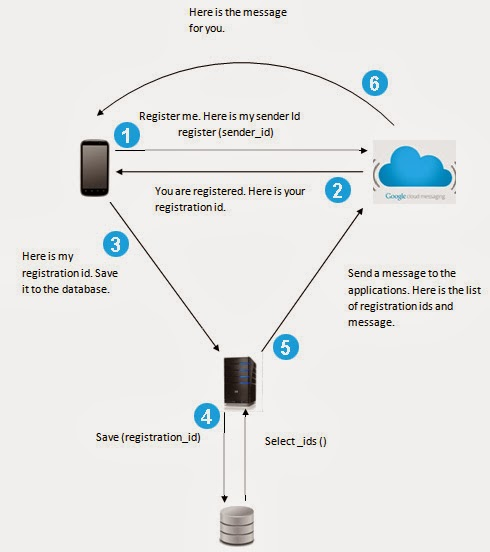
\includegraphics[scale=0.8]{GCM}
\caption{GCM System Architecture}
\label{fig:GCM}
\end{center}
\end{figure}

\section {Key Concepts of GCM}

\subsection {GCM Components}
\begin {enumerate}
  \item\textbf { Client App} – It is a GCM-enabled Android application running on a device. This must be 2.2+ Android OS device with Google Play Store installed, and it must have at least one logged in Google account if the device is running a version lower than Android 4.0.4.

   \item\textbf { 3rd party Application Server }– An application server that you write as part of implementing GCM. The 3rd-party application server sends data via the GCM connection server to Android application on the device.

    \item\textbf {GCM Connection Server} – These are Google-provided servers involved in taking messages from the 3rd-party application server and sending them to the device.

\end {enumerate}

\subsection {GCM Credentials}
\begin {enumerate}
  \item\textbf {Sender ID} – The sender ID is used in the registration process to identify a 3rd-party application server that is permitted to send messages to the device.

    \item\textbf{Application ID} – The Android application that is registering to receive messages.

    \item\textbf {Registration ID } – An ID issued by the GCM servers to the Android application that allows it to receive messages. Once the Android application has the registration ID, it sends it to the 3rd-party application server, which uses it to identify each device that has registered to receive messages for a given Android application.
    
 \item\textbf {    Sender Auth Token} – An API key that is saved on the 3rd-party application server that gives the application server authorized access to Google services. The API key is included in the header of POST requests that send messages.
\end {enumerate}

\section{Life Cycle Flow}
\begin{enumerate}
   \item\textbf {Enable GCM} – Android application running on a mobile device registers to receive messages. To use the messaging service on Android application for the first time, it needs to call the GoogleCloudMessaging method register(). The register() method returns a registration ID which should be stored by our Android application for later use.
   
   \item\textbf {Send A Message} – A 3rd-party application server sends messages to the device. Here is the sequence of events that occurs when the application server sends a message. Message is sent to GCM servers by the application server. Google enqueues and stores the message incase the device is offline. When the device is online, Google sends the message to the device. On the device, the system broadcasts the message to the specified Android application via Intent broadcast with proper permissions, so that only the targeted Android application gets the message. This wakes the Android application up. The Android application does not need to be running beforehand to receive the message. 
   
   The Android application processes the message. If the Android application is doing non-trivial processing, you may want to grab a PowerManager WakeLock and do any processing in a service. The Android application extracts the raw data from the com.google.android.c2dm.intent.RECEIVE Intent by key and processes the data.
        
   \item\textbf {Receive A Message} – Android application receives a message from GCM server. This is the sequence of events that occurs when an Android application installed on a mobile device receives a message.
   
   \begin{enumerate}
      \item  The system receives the incoming message and extracts the raw key/value pairs from the message payload, if any.
      \item The system passes the key/value pairs to the targeted Android application in a com.google.android.c2dm.intent.RECEIVE Intent as a set of extras.
   \end{enumerate}



\end{enumerate}


\chapter{Epilogue}

\section{Challenges}
\begin{enumerate}
\item Multi-Lingual Support for the local language spoken by community people.
\item Design in coherence with end user capabilities to minimize user input on the GUI and increase its usability.
\item Capturing user requirements
\item Content Management and Content Moderation
\item Understanding the design structure of Gram Vaani, the methology of managing surveys, their mapping and creation.
\item Data security and data moderation regarding the information of the users
\item Scalability of the application
\end{enumerate}

\section{Conclusions}

\begin{enumerate}
\item Main issues and problems are specific to the villages, to the regions. They
need to be identified and then application can be used and make a great
contribution in actually helping people by various means.
\item Manual intervention and involvements are the key elements in introducing
big changes and turning heads of the people.
\item The local knowledge of village is very important prior introducing any new
model in that place.
\item Necessity of responsible people in various regulatory authorities, commission
departments, panchayats, Government officers, NGO’s workers, ASHA
workers, school teachers.
\item Application is designed for both the Hindi and English application users.
\item Web Portal interface is designed for the NGO personnels.
\item The surveys and other functionalities will help in dissemination of information effectively.
\end{enumerate}


\section{Future Work}

\begin{enumerate}
\item \textbf{Deployment of Mobile Application} - Mobile Application will be deployed in the community where volunteers will be provided with the pre loaded .apk file with the android phones. Volunteers’ feedback will be analysed and incorporated to increase the usability of the application. Volunteers should be given timely trainings regarding the usage of application and other uses  of basic phone must be taught.
\item \textbf{Creating Surveys from Application} - Feature of creating a new survey, adding questions, uploading audio prompts etc  can be added in the application for volunteers as well as on the portal for the NGO users.
\item \textbf{Sending Announcements and Messages from Portal} - NGO user can record audio announcements and can send instant text messages to the volunteers on their mobile phones. 
\end{enumerate}






\bibliographystyle{plain}
\bibliography{biblio}

\appendix
\chapter{Screenshots of the 'Gologo' Application}

Following screenshots depict the graphical user interface of the application.

\begin {enumerate}
\item First time Application Users will be authenticated via PIN received through the message when NGO registers through the portal.
\begin{figure}[H]
\begin{center}   
\includegraphics[scale=0.4]{Loginscreen}
\caption{Pin Authentication}
\label{fig:pin_authenticate}
\end{center}
\end{figure}

\item Online User Registration by the NGO sends a message on registered number for authentication.
\begin{figure}[H]
\begin{center}   
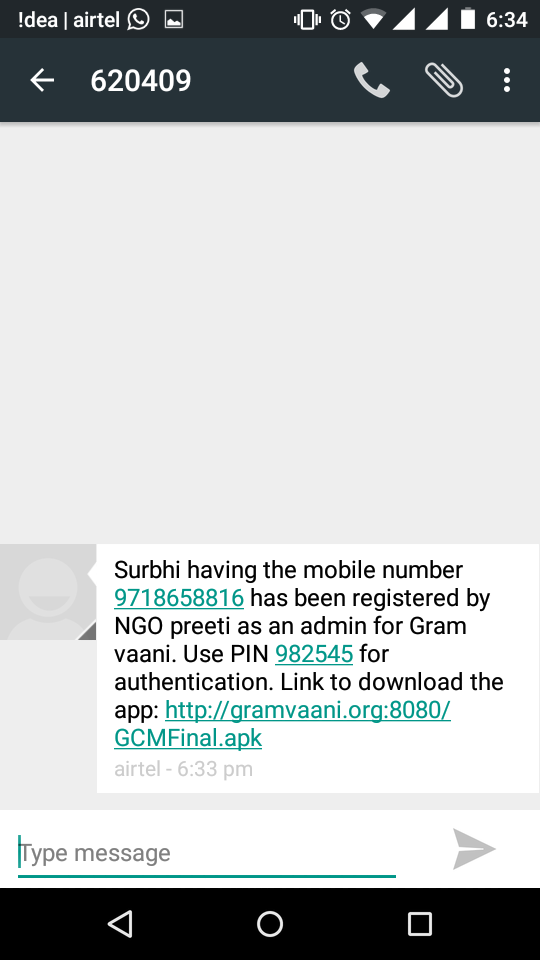
\includegraphics[scale=0.26]{authenticatemsg}
\caption{Message for Pin Authentication}
\label{fig:authenticatemsg}
\end{center}
\end{figure}

\item User can retrieve PIN by clicking on Forget PIN option.
\begin{figure}[H]
\begin{center}   
\includegraphics[scale=0.4]{Pinrecovery}
\caption{Pin Recovery}
\label{fig:pin_recovery}
\end{center}
\end{figure}

\item User will be provided with the following options.
\begin{figure}[H]
\begin{center}   
\includegraphics[width=0.8\textwidth]{Workflowapp}
\caption{Use Cases}
\label{fig:menuoptions}
\end{center}
\end{figure}

\item User can record audio by recording audio using Media Recorder.
\begin{figure}[H]
\begin{center}   
\includegraphics[scale=0.4]{Audiorecord}
\caption{Record Audio}
\label{fig:audio1}
\end{center}
\end{figure}

\item User can send instant text messages by choosing any of the below template depending upon the type of announcement.
\begin{figure}[H]
\begin{center}   
\includegraphics[scale=0.42]{Msgtemplates}
\caption{Type of Text Announcements}
\label{fig:message}
\end{center}
\end{figure}

\item Text alert of survey to be launched in the community will be sent with the specified date to inform people regarding the survey launch.
\begin{figure}[H]
\begin{center}   
\includegraphics[scale=0.44]{surveytemplate}
\caption{Announcement of Surveys}
\label{fig:message1}
\end{center}
\end{figure}

\item Text alert of upcoming camp to be organised in the community will be sent with the specified parameters to inform people. 
\begin{figure}[H]
\begin{center}   
\includegraphics[scale=0.4]{camptemplate}
\caption{Announcement of Camps}
\label{fig:message2}
\end{center}
\end{figure}


\item  Launched scheme name along with the details of scheme date and beneficiaries for that scheme will be sent to the target people to send text alerts to inform people regarding it.
\begin{figure}[H]
\begin{center}   
\includegraphics[scale=0.4]{schemetemplate}
\caption{Announcement of Govt. Schemes}
\label{fig:message3}
\end{center}
\end{figure}

\item The app users can add a new contact. The user selects the option of Add a contact on the  home screen of application. In this option, he can fill in all the details of a new contact of his community having name, contact number, gender, date of birth, contact groups and location URI.
\begin{figure}[H]
\begin{center}   
\includegraphics[scale=0.4]{Addcontact}
\caption{Add a New Contact}
\label{fig:contact1}
\end{center}
\end{figure}

\item In the above option, application user is asked for the confirmation via a diaglog box. He can either click on confirm for adding a new contact or cancel the adding of contact.
\begin{figure}[H]
\begin{center}   
\includegraphics[scale=0.4]{contactconfirm}
\caption{Confirmation Screen while Adding Contact}
\label{fig:contact2}
\end{center}
\end{figure}
 
\item  Volunteers are given this functionality for the management of contact groups. Multiple contact groups are made and managed as per the groups of the community. It helps in easy dissemination of information to the relevant audience.
\begin{figure}[H]
\begin{center}   
\includegraphics[scale=0.4]{addgroup}
\caption{Add a New Contact Group}
\label{fig:group1}
\end{center}
\end{figure}

\item Application user can view the active survey of the GramVaani Server corresponding to the application instance.
\begin{figure}[H]
\begin{center}   
\includegraphics[scale=0.42]{launchsurvey}
\caption{List of Active Surveys}
\label{fig:viewlaunchsurvey}
\end{center}
\end{figure}

\item Application user can view a particular survey with all the survey questions along with the type of question. One can also listen the audio prompt of each survey question.
\begin{figure}[H]
\begin{center}   
\includegraphics[scale=0.42]{surveyques}
\caption{View a Particular Survey}
\label{fig:viewsurvey}
\end{center}
\end{figure}

\item  Application user can choose the target people among the Gramvaani groups, his phone callers and  Mobile Vaani instance callers.
\begin{figure}[H]
\begin{center}   
\includegraphics[scale=0.42]{sendoptions}
\caption{Choose Contact Options to Launch}
\label{fig:contactoptions}
\end{center}
\end{figure}

\item Multiple Gramvaani contact groups can be choosen as the target audience.
\begin{figure}[H]
\begin{center}   
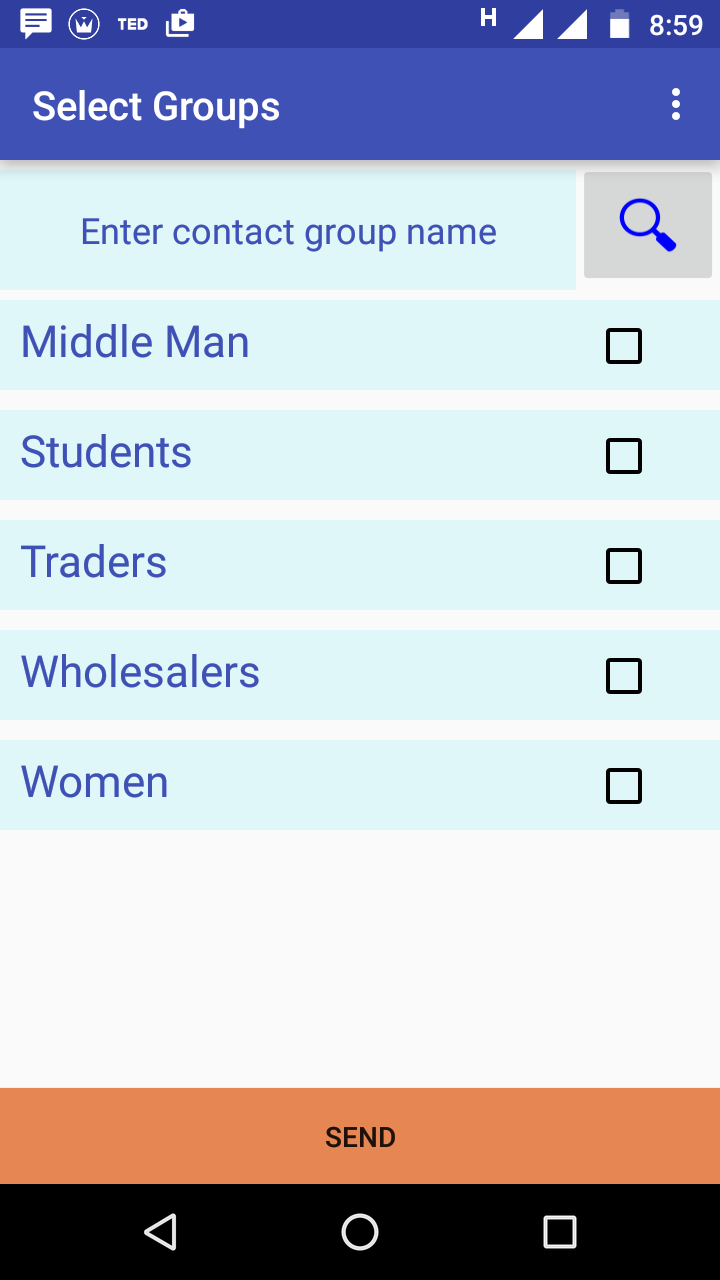
\includegraphics[scale=0.18]{contactgroups}
\caption{GV Contact Groups}
\label{fig:contactgroups}
\end{center}
\end{figure}

\item Multiple phone contacts can be choosen as the target people.
\begin{figure}[H]
\begin{center}   
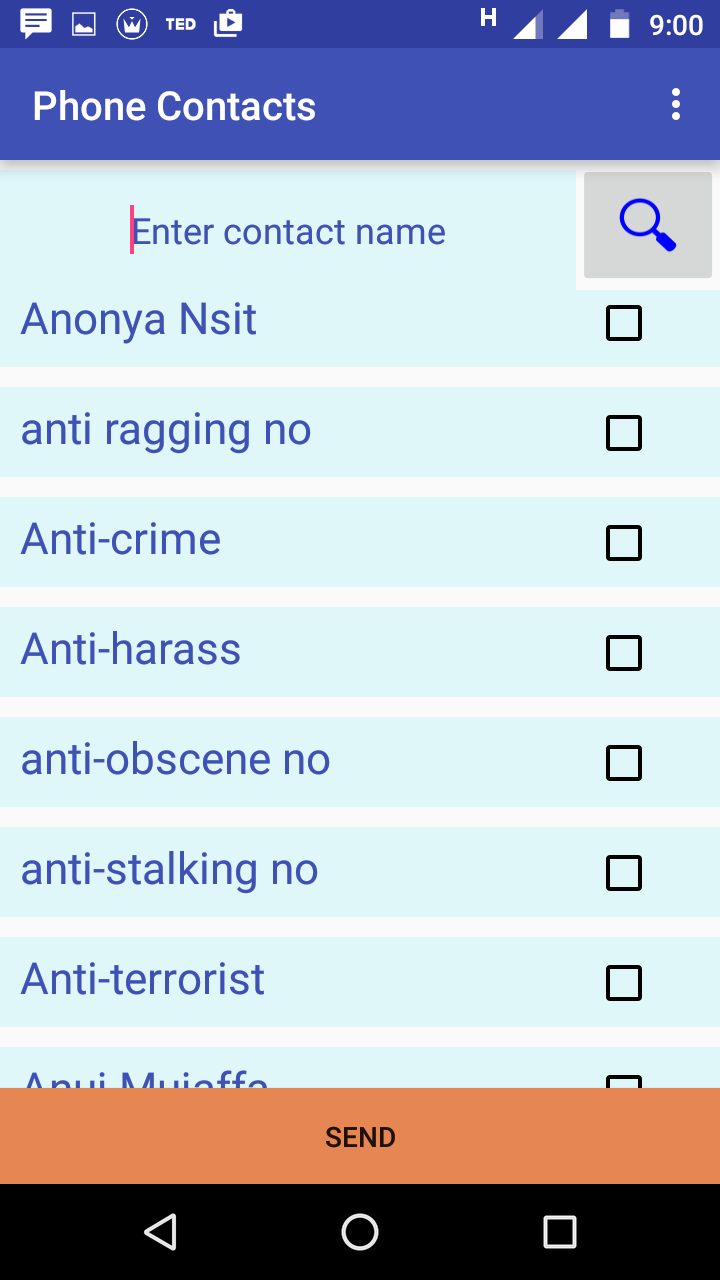
\includegraphics[scale=0.16]{phonecontacts}
\caption{Phone Contacts}
\label{fig:phonecontacts}
\end{center}
\end{figure}

\item Some quick options are provided on the application which are available across all activities. Application  user can navigate across these options.
\begin{figure}[H]
\begin{center}   
\includegraphics[scale=0.4]{Actionbaroptions}
\caption{Options on Menu Bar}
\label{fig:menubar}
\end{center}
\end{figure}

\end{enumerate}





\chapter{Screenshots of the Web Portal}

%\begin{enumerate}
\begin{figure}[H]
    \centering
	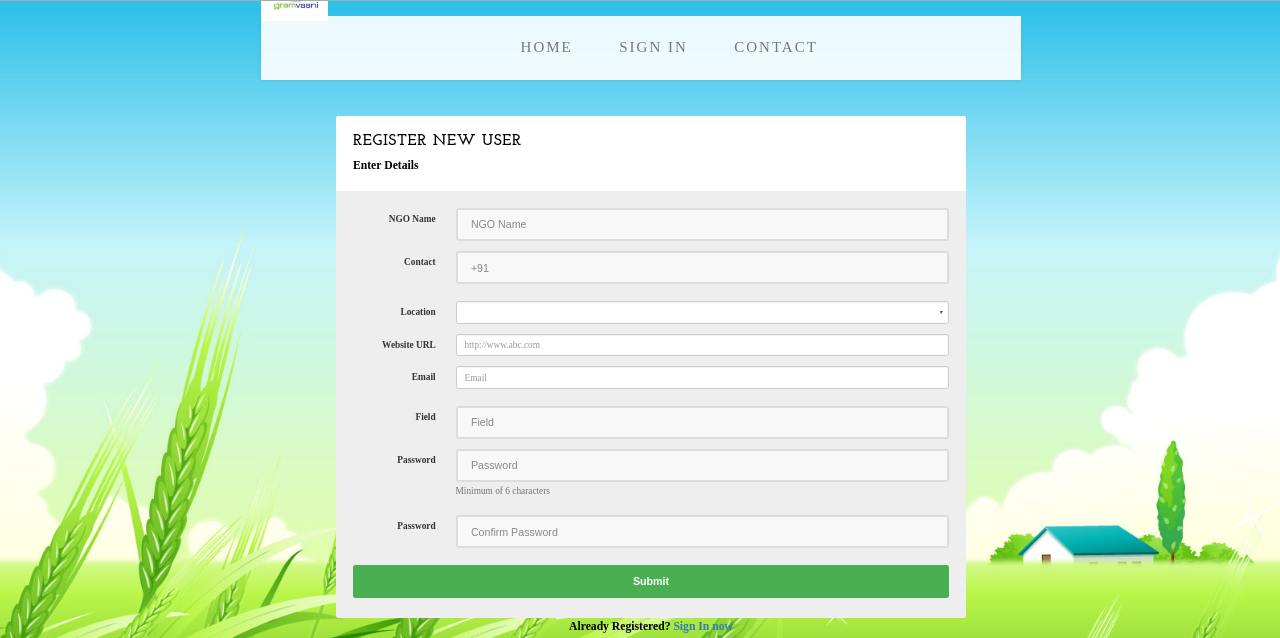
\includegraphics[width=1\textwidth]{RegisterNGOuser.png}
    \caption{Register new NGO user on the Web Portal}
    \label{fig:Register new NGO user on the Web Portal}
\end{figure}

\begin{figure}[H]
    \centering
	
\includegraphics[width=1\textwidth]{AfterSignInHomepage.png}
    \caption{Home Page After Login on the Web Portal}
    \label{fig:Home Page After Login on the Web Portal}
\end{figure}


\begin{figure}[H]
    \centering
	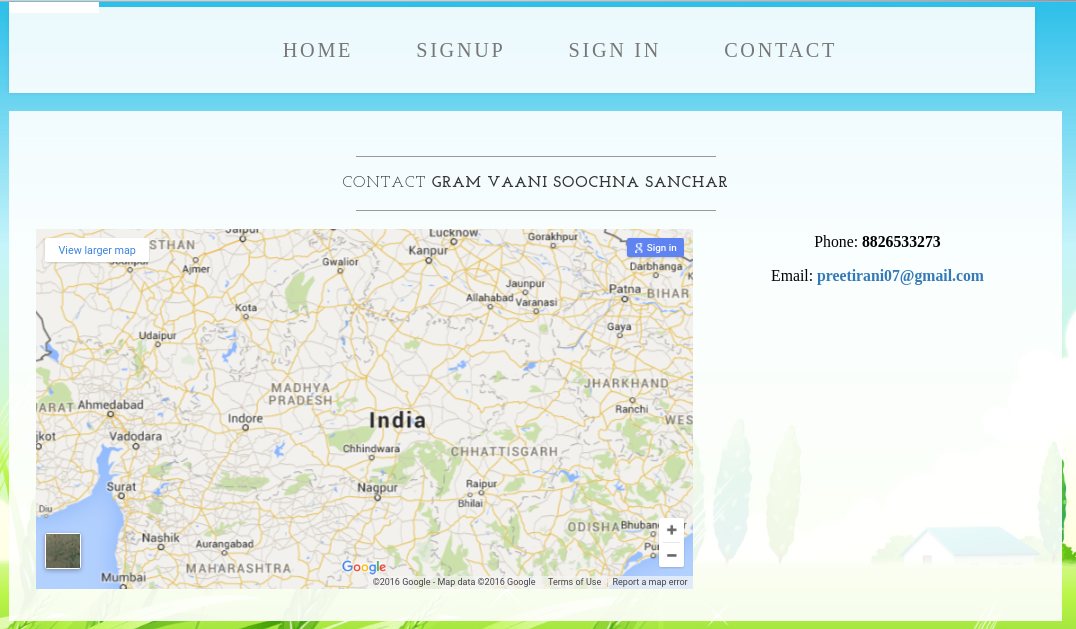
\includegraphics[width=1\textwidth]{ContactPage.png}
    \caption{Contact Gramvaani Page on the Web Portal}
    \label{fig:Contact Gramvaani Page on the Web Portal}
\end{figure}

\begin{figure}[H]
    \centering
	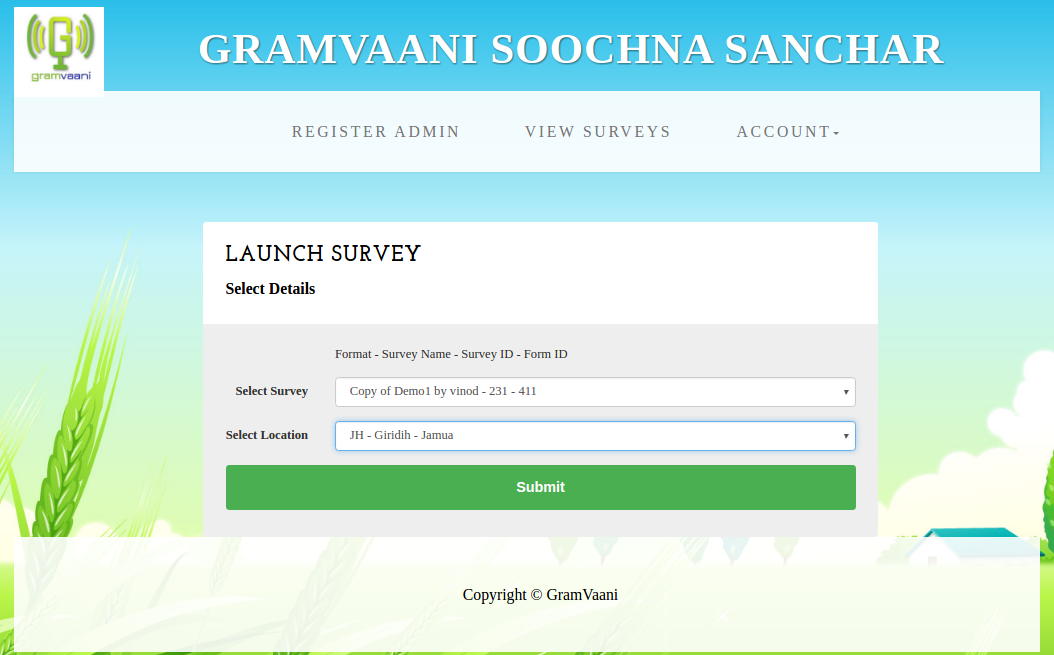
\includegraphics[width=1\textwidth]{LaunchSurvey1.png}
    \caption{Launch Survey Step 1 on the Web Portal}
    \label{fig:Launch Survey Step 1 on the Web Portal}
\end{figure}

\begin{figure}[H]
    \centering
	\includegraphics[width=1\textwidth]{LaunchSurvey2.png}
    \caption{Launch Survey Step 2 on the Web Portal}
    \label{fig:Launch Survey Step 2 on the Web Portal}
\end{figure}

\begin{figure}[H]
    \centering
	\includegraphics[width=1\textwidth]{LaunchSurvey3.png}
    \caption{Launch Survey Step 3 on the Web Portal}
    \label{fig:Launch Survey Step 3 on the Web Portal}
\end{figure}

\begin{figure}[H]
    \centering
	\includegraphics[width=1\textwidth]{ListenAudioPrompt}
    \caption{Listen Question Audio Prompt on the Web Portal}
    \label{fig:Listen Question Audio Prompt on the Web Portal}
\end{figure}


\begin{figure}[H]
    \centering
	\includegraphics[width=1\textwidth]{Logintothesiteautofillcredentials.png}
    \caption{Login into the Web Portal}
    \label{fig:Login into the Web Portal}
\end{figure}


\begin{figure}[H]
    \centering
	\includegraphics[width=1\textwidth]{NGOUserProfile.png}
    \caption{View Logged in User Profile on the Web Portal }
    \label{fig:View Logged in User Profile on the Web Portal}
\end{figure}

\begin{figure}[H]
    \centering
	\includegraphics[width=1\textwidth]{PortalHomepagePart1.png}
    \caption{Homepage part 1 on the Web Portal}
    \label{fig:Homepage part 1 on the Web Portal}
\end{figure}

\begin{figure}[H]
    \centering
	\includegraphics[width=1\textwidth]{PortalHomepagePart2.png}
    \caption{Homepage part 2 on the Web Portal}
    \label{fig:Homepage part 2 on the Web Portal}
\end{figure}

\begin{figure}[H]
    \centering
	\includegraphics[width=1\textwidth]{PortalHomepagePart3.png}
    \caption{Homepage part 3 on the Web Portal}
    \label{fig:Homepage part 3 on the Web Portal}
\end{figure}

\begin{figure}[H]
    \centering
	\includegraphics[width=1\textwidth]{RegisterAdmin1.png}
    \caption{Register new admin step 1 on the web portal}
    \label{fig:Register new admin step 1 on the web portal}
\end{figure}

\begin{figure}[H]
    \centering
	\includegraphics[width=1\textwidth]{RegisterAdmin2.png}
    \caption{Register new admin step 2 on the web portal}
    \label{fig:Register new admin step 2 on the web portal}
\end{figure}

\begin{figure}[H]
    \centering
	\includegraphics[width=1\textwidth]{ViewResponses.png}
    \caption{View Survey Responses on the Web Portal}
    \label{fig:View Survey Responses on the Web Portal}
\end{figure}

\begin{figure}[H]
    \centering
	\includegraphics[width=1\textwidth]{ViewSurveyQuestions.png}
    \caption{View Survey Questions on the Web Portal}
    \label{fig:View Survey Questions on the Web Portal}
\end{figure}


\begin{figure}[H]
    \centering
	\includegraphics[width=1\textwidth]{ViewSurveys.png}
    \caption{View Surveys on the Web Portal}
    \label{fig:View Surveys on the Web Portal}
\end{figure}

%\end{enumerate}
\chapter{Screenshots of Gramvaani GUI}




\begin{figure}[H]
\begin{center}   
\includegraphics[scale=0.3]{aisurvey}
\caption{GramVaani Web Instance Surveys}
\label{fig:gvinstance1}
\end{center}
\end{figure}



\begin{figure}[H]
\begin{center}   
\includegraphics[scale=0.3]{aimv}
\caption{Mobile Vaani Items}
\label{fig:gvinstance2}
\end{center}
\end{figure}



\begin{figure}[H]
\begin{center}   
\includegraphics[scale=0.3]{aiitems}
\caption{Published items on GramVaani Web Instance}
\label{fig:gvinstance3}
\end{center}
\end{figure}



\begin{figure}[H]
\begin{center}   
\includegraphics[scale=0.3]{aicontacts}
\caption{GramVaani Contact Groups along with Contacts}
\label{fig:gvinstance4}
\end{center}
\end{figure}


















\end {document}
	